\chapter{Theoretical Calculations}
\label{chap:Theory_Predictions}

In an experiment, the measurements are validated by doing the comparison with the perturbative QCD (pQCD) theoretical calculations. The lowest order (LO) calculations describe well the shapes of the measured distributions but not the normalization due to the dependence on the unphysical renormalization (\mur) and factorization (\muf) scales. The next-to-leading order calculations (NLO) improves the precision by reducing the dependence on \mur and \muf scales and become an essential feature in the determination of fundamental parameters such as $\alpha_S$ and the parton density distributions. In this chapter, the next-to-leading order pQCD calculations are described in details. NLO pQCD calculations are corrected for the multiparton interactions (MPI) and hadronisation effects by applying non-perturbative (NP) corrections and also corrected for the electroweak interactions (EW).

\section{Fixed order NLO calculations}
The predictions of the inclusive differential jet event cross section at NLO accuracy in pQCD are computed with the \NLOJETPP program version~4.1.3~\cite{Nagy:2001fj,Nagy:2003tz}. The results are provided within the framework of \fastNLO version~2.3~\cite{Kluge:2006xs,Britzger:2012bs} for use within fits. The parton distribution functions (PDFs) are accessed through the \LHAPDFS library \cite{Whalley:2005nh,Buckley:2014ana}. The \fastNLO is preferred over the direct calculation with \NLOJETPP as the calculations of the cross sections can be repeated several times with different PDFs as well as scale choices required for the calculating PDF and scale uncertainties. The renormalization and factorization scales are chosen equal to \httwo, i.e. \mur = \muf = \httwo. 

In the current study, different PDF sets available for a series of different assumptions on \alpsmz are used for NLO calculations. In Table~\ref{tab:chap2:nlopdfsets}, already existing PDF sets in LHC Run~1 (upper rows) and newer ones for Run~2 (lower rows) are listed together with the corresponding number of flavours $N_f$, the assumed masses $M_t$ and $M_Z$ of the top quark and the $Z$ boson, respectively, the default values of \alpsmz, and the range in \alpsmz variation available for fits. All sets employ a variable-flavour number scheme with at most five or six flavours apart from the ABM11 PDFs, which use a fixed-flavour number scheme with $\NF=5$. Out of these eight PDF sets the following three are not considered further beacuse of the below mentioned reasons :

\begin{itemize}
\item At NLO, predictions based on ABM11 do not describe LHC jet data at small jet rapidity \cite{Aad:2013lpa, Aad:2014vwa, CMS:2014mna, Khachatryan:2015luy}.
\item The HERAPDF2.0 set exclusively fits HERA DIS data with only weak constraints on the gluon PDF.
\item The range in values available for \alpsmz is too limited for the NNPDF3.0 set.
\end{itemize}

\begin{table}[htbp]
 \centering
 \caption{NLO PDF sets are available via \LHAPDFS with various assumptions on the value of \alpsmz. The already existing sets in LHC Run~1 (upper rows) and newer ones for Run~2 (lower rows) are listed here with the corresponding number of flavours $N_f$, the assumed masses $M_t$ and $M_Z$ of the top quark and the $Z$ boson, respectively, the default values of \alpsmz, and the range in \alpsmz variation available for fits.  A~$^*$ behind the \alpsmz values signifies that the parameter was fixed, not fitted.}
 \label{tab:chap2:nlopdfsets}
 \vspace{2mm}
 \begin{tabular}{lccllc}
 \hline\hline
 Base set & \NF & $M_t$ (\GeVns{}) & $M_Z$ (\GeVns{}) &\alpsmz & \alpsmz range\rbthm\\  \hline
 % LHC Run 1
 ABM11    \cite{Alekhin:2012ig} &  5   & 180       & 91.174  & $0.1180$   & 0.110--0.130\rbtrr\\
 CT10     \cite{Lai:2010vv}     & ${\leq}5$ & 172       & 91.188  & $0.1180^*$ & 0.112--0.127\rbtrr\\
 MSTW2008 \cite{Martin:2009iq,Martin:2009bu} & ${\leq}5$ & $10^{10}$ & 91.1876 & $0.1202$   & 0.110--0.130\rbtrr\\
 NNPDF2.3 \cite{Ball:2012cx} & ${\leq}6$ & 175       & 91.1876 & $0.1180^*$ & 0.114--0.124\rbtrr\\\hline
 % LHC Run 2
 CT14     \cite{Dulat:2015mca} & ${\leq}5$ & 172       & 91.1876 & $0.1180^*$ & 0.113--0.123\rbtrr\\
 HERAPDF2.0 \cite{Abramowicz:2015mha} & ${\leq}5$ & 173       & 91.1876 & $0.1180^*$ & 0.110--0.130\rbtrr\\
 MMHT2014 \cite{Harland-Lang:2014zoa} & ${\leq}5$ & $10^{10}$ & 91.1876 & $0.1180^*$ & 0.108--0.128\rbtrr\\
 NNPDF3.0 \cite{Ball:2014uwa} & ${\leq}5$ & 173       & 91.2    & $0.1180^*$ & 0.115--0.121\rbtrr\\
 \hline\hline
 \end{tabular}
\end{table}

\subsection{NLO Correction Factors}
\label{sec:nlo_factors}
The differences between LO predictions and NLO predictions give the impact of the higher-order contributions to the pQCD predictions. These are described by a NLO correction factor, k\hy factor, which is defined as the ratio of cross sections at NLO accuracy to that at LO i.e.

\begin{equation}
\label{eq:kfactors}
 {\rm k\hy factor} = \frac{\sigma_{\rm NLO}}{\sigma_{\rm LO}}
\end{equation}
%i.e. ${\rm k\hy factor}_{\ratio} = {\rm \frac{k\hy factor_{3\hy jet}}{k\hy factor_{2\hy jet}}}$. 
The size of k-factor determine the effect of the higher-order corrections. The small size of k-factor indicates that the cross section predictions are precisely described at the LO whereas the larger size hints the contributions from NLO. Figure~\ref{fig:kfactor} shows the k-factors of the \NLOJETPP calculations, for inclusive 2-jet and 3-jet events cross sections and their ratio \ratio, using five different PDF sets. k-factor for \ratio is obtained by taking the ratio of k-factors for inclusive 3-jet events cross sections to that of inclusive 2-jet. The k-factors are similar for all the PDF sets in the lower region, but the differences increase in regions with larger \httwo. It is observed that for inclusive 3-jet events cross sections, k-factor jumps at lowest \httwo. This is because some jet configurations are kinematically forbidden near the \pt cut bin i.e. 150 GeV. Since the first few bins in \httwo (below 225 GeV) still suffer from these kinematical effects, the minimum value of \httwo studied is 300 GeV.

\begin{figure}[!htbp]
 \begin{center}
 \hspace*{-5mm}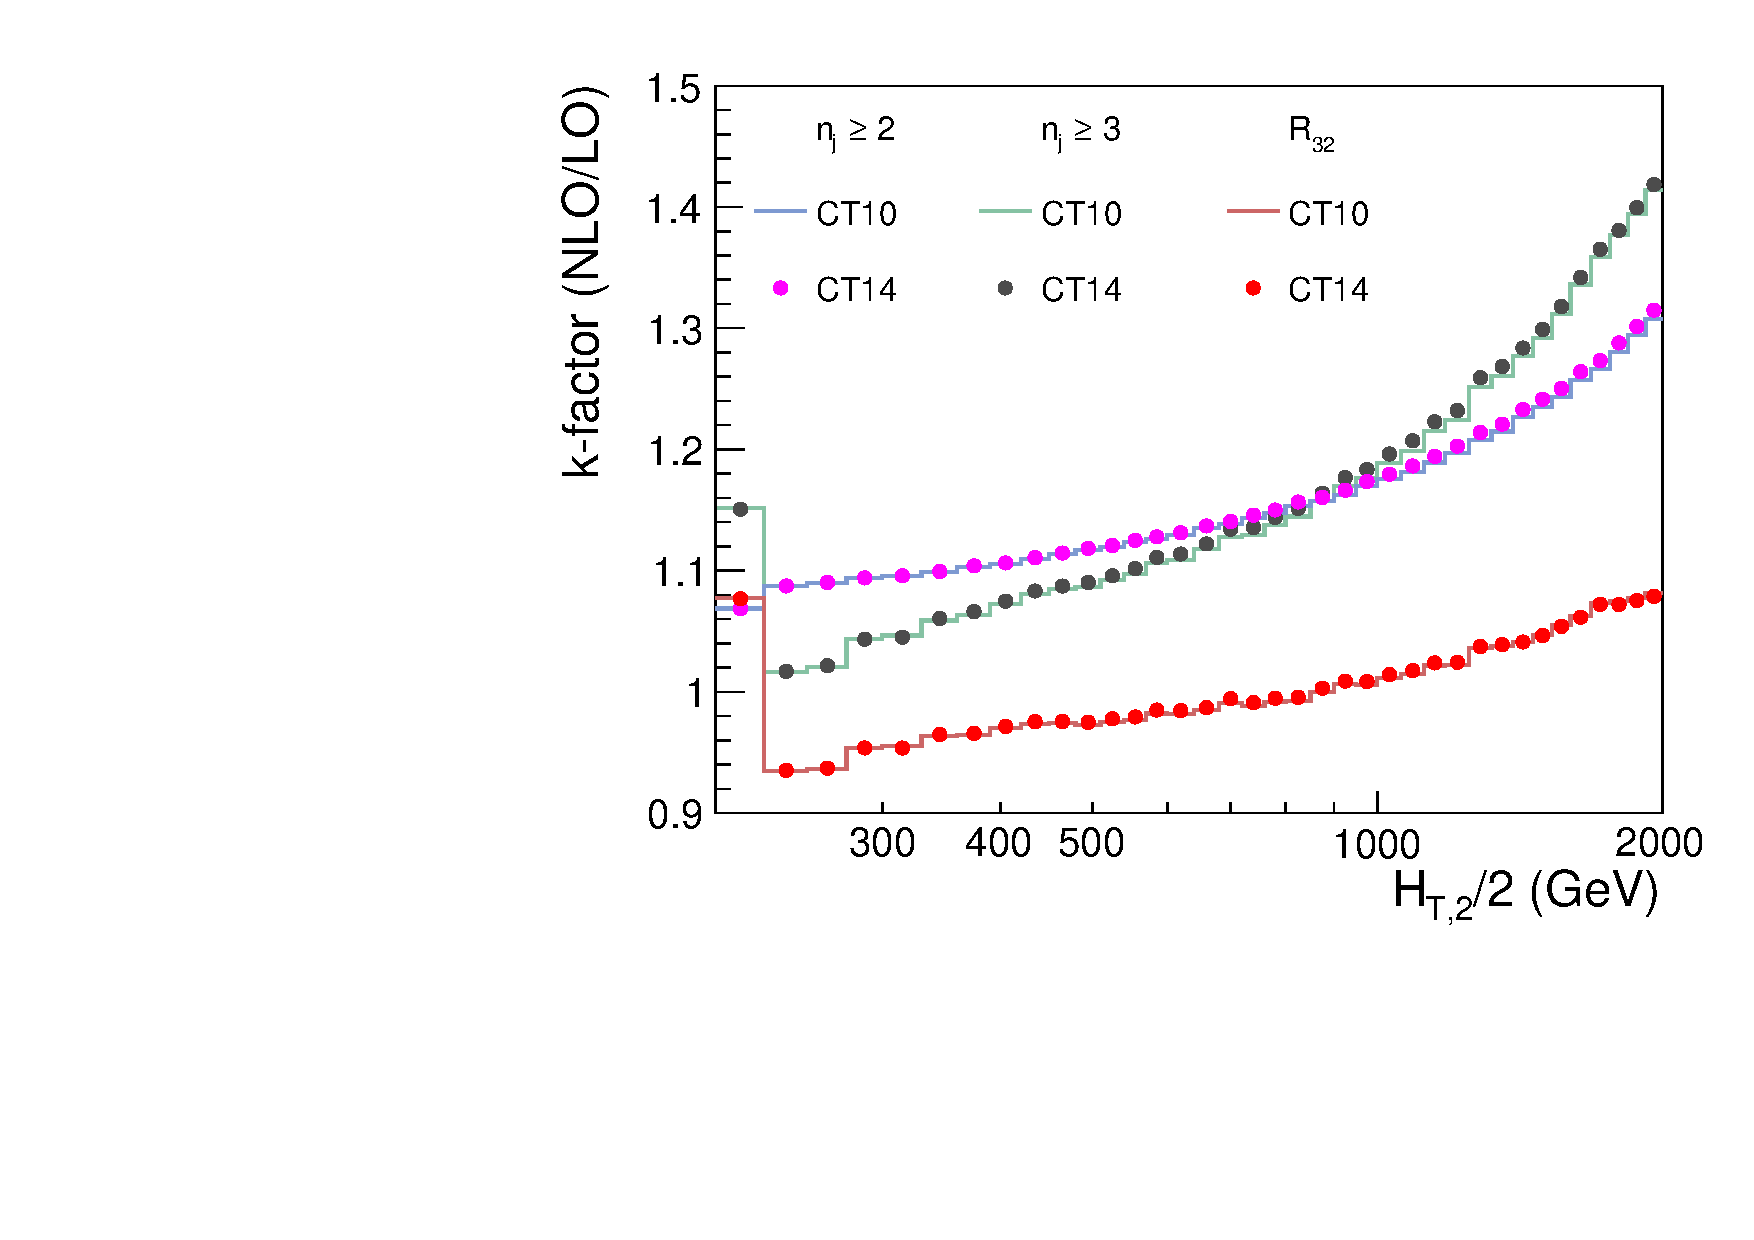
\includegraphics[width=0.51\textwidth]{Plots_HT_2_150/Kfactor_all_1.pdf}%
 ~~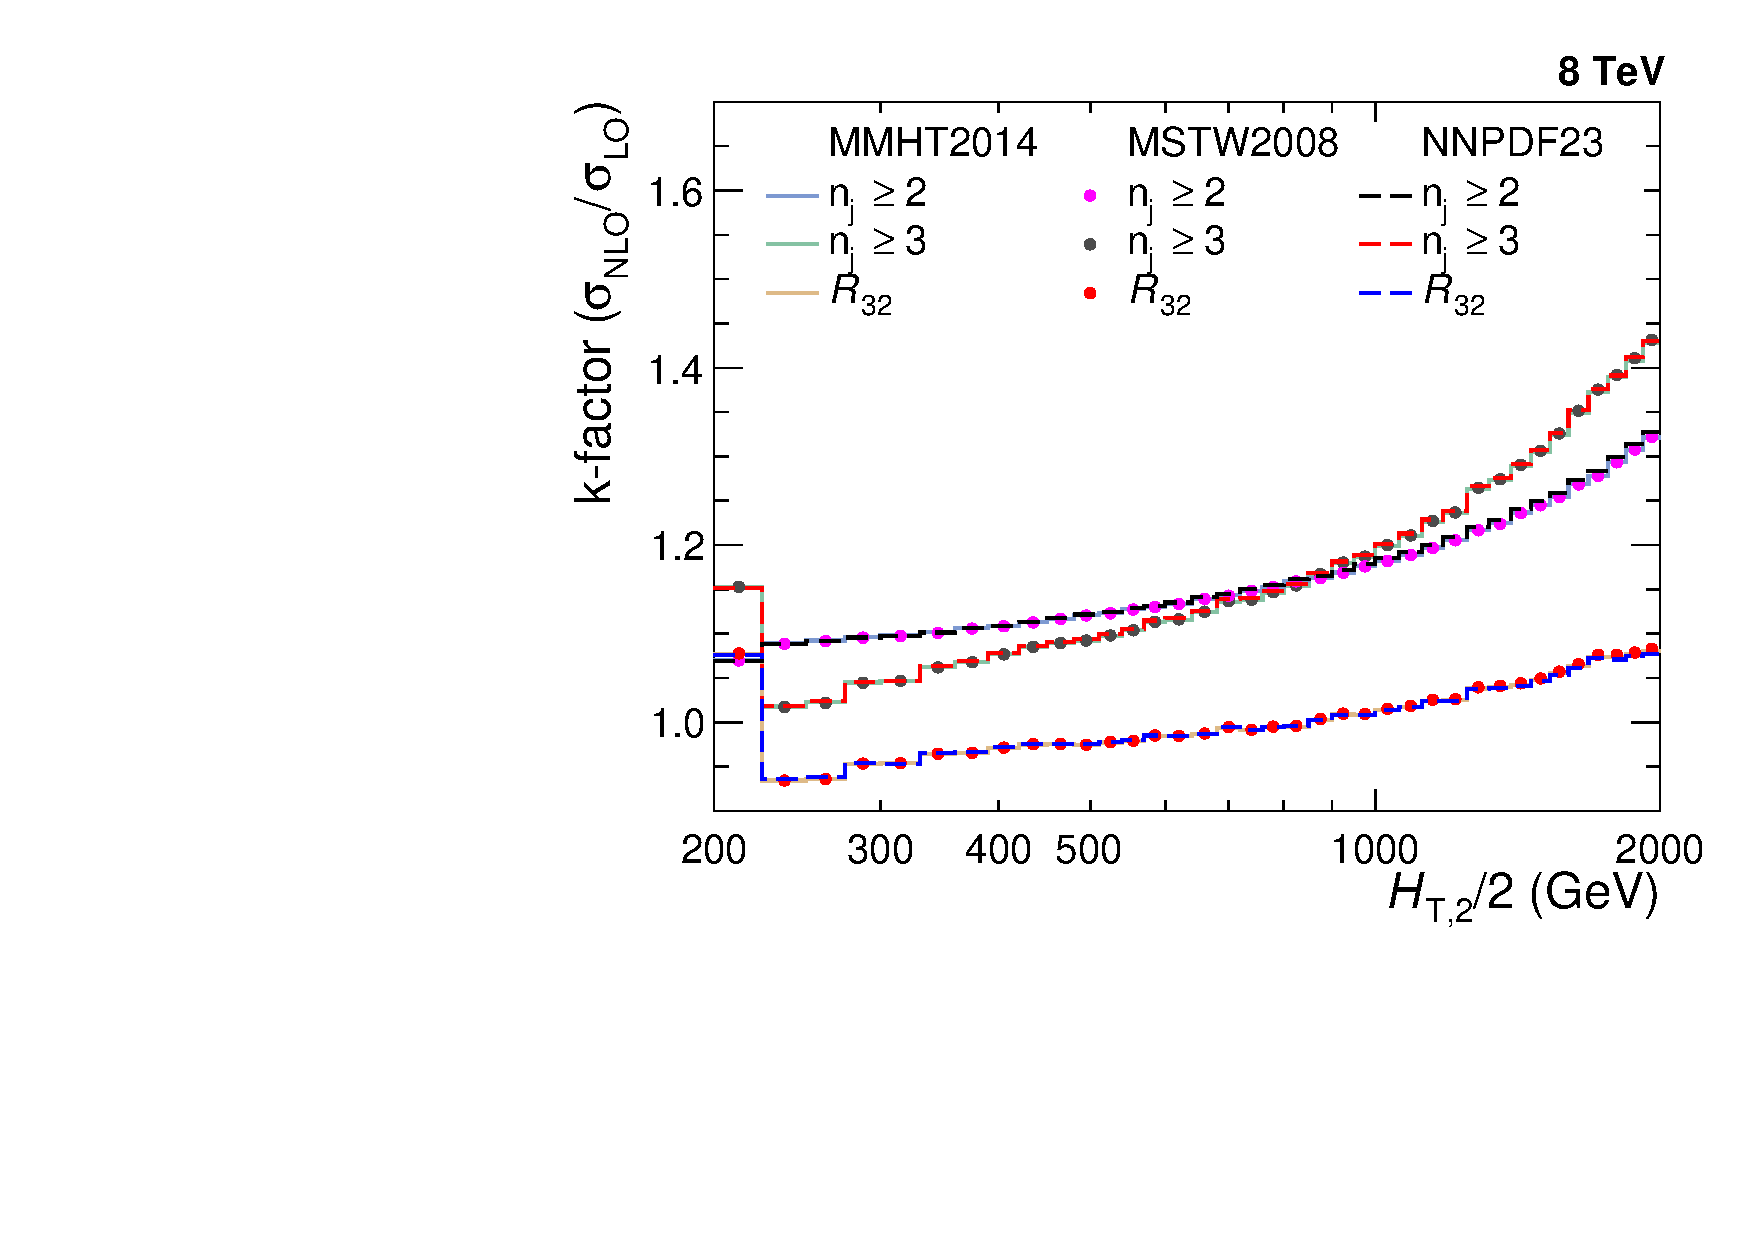
\includegraphics[width=0.51\textwidth]{Plots_HT_2_150/Kfactor_all_2.pdf}
 \caption{The k-factors of the \NLOJETPP calculations, for inclusive 2-jet and 3-jet events cross sections and their ratio \ratio, using five different PDF sets.}
  \label{fig:kfactor}
  \end{center}
\end{figure}

\subsection{Non-Perturbative Corrections}
\label{sec:NPcorr}
The fixed-order pQCD calculations predict the parton-level cross section and do not include additional soft QCD effects and hence cannot be directly compared to unfolded data. These calculations should be corrected for non-perturbative effects (NP) before comparison with the measurement at particle level. The impact of NP effects, \ie from multiple-parton interactions (MPI) and hadronization, are evaluated by using samples obtained from different MC event generators with a simulation of parton-shower and underlying-event (UE) contributions. The leading order (LO), \HERWIGPP~\cite{Bahr:2008pv} with the default tune of version 2.3 and \PYTHIAS~\cite{Sjostrand:2006za} with tune \Ztwostar, and the NLO, \POWHEG~\cite{Nason:2004rx,Frixione:2007vw,Alioli:2010xa}, MC event generators are considered. The matrix-element calculation performed with \POWHEG is interfaced to \PYTHIAE with tune CUETM1~\cite{Khachatryan:2015pea} for the UE simulation. The cross section ratios between a nominal event generation interfaced to the simulation of UE contributions and a sample without hadronization and MPI effects are taken as correction separately for inclusive 2-jet, 3-jet events and ratio \ratio, defined as in Equation~\ref{Eq:np}. Equation~\ref{Eq:np_ratio} is used to calculate the NP correction factor for \ratio. The correction is then applied as a bin-by-bin correction factor to the parton-level NLO cross section. 

\begin{equation}
  \label{Eq:np}
  C^{NP} = \frac{\sigma^{PS\texttt{+}HAD\texttt{+}MPI}}{\sigma^{PS}}
\end{equation}


\begin{equation}
  \label{Eq:np_ratio}
  C^{NP}_{\ratio} = \frac{\Big(\frac{\sigma_{3\mbox{-}jet}}{\sigma_{2\mbox{-}jet}}\Big)^{PS\texttt{+}HAD\texttt{+}MPI}}{\Big(\frac{\sigma_{3\mbox{-}jet}}{\sigma_{2\mbox{-}jet}}\Big)^{PS}}
\end{equation}

\begin{equation}
  \label{Eq:power}
  f(\httwo) = a\cdot\big(\httwo\big)^{b}\texttt{+}~c
\end{equation}

This ratio is fitted by a power-law function defined in Equation~\ref{Eq:power}. Since the correction factors obtained from different MC generators have large differences, an uncertainty is assigned to the correction factor. The correction factors $C^{\mathrm{NP}}$ are determined by the average of the envelope which covers all the differences and half of it is taken as the uncertainty. The NP corrections are shown in Figure~\ref{fig:np_factors} for the inclusive 2-jet (top left) and 3-jet event cross sections (top right), as well as for ratio \ratio (bottom). They amount to $\sim$ 5\% for inclusive 2-jet, $\sim$ 7--8\% for inclusive 3-jet events and $\sim$ 4\% for ratio \ratio, for \httwo $\sim$ 200 GeV and decrease rapidly for increasing \httwo. The uncertainty assigned to the NP corrections is of the order of 1--2\%. The non-perturbative effects are reduced in the cross section ratio.

\begin{figure}[!htbp]
 \begin{center}
 \hspace*{-5mm}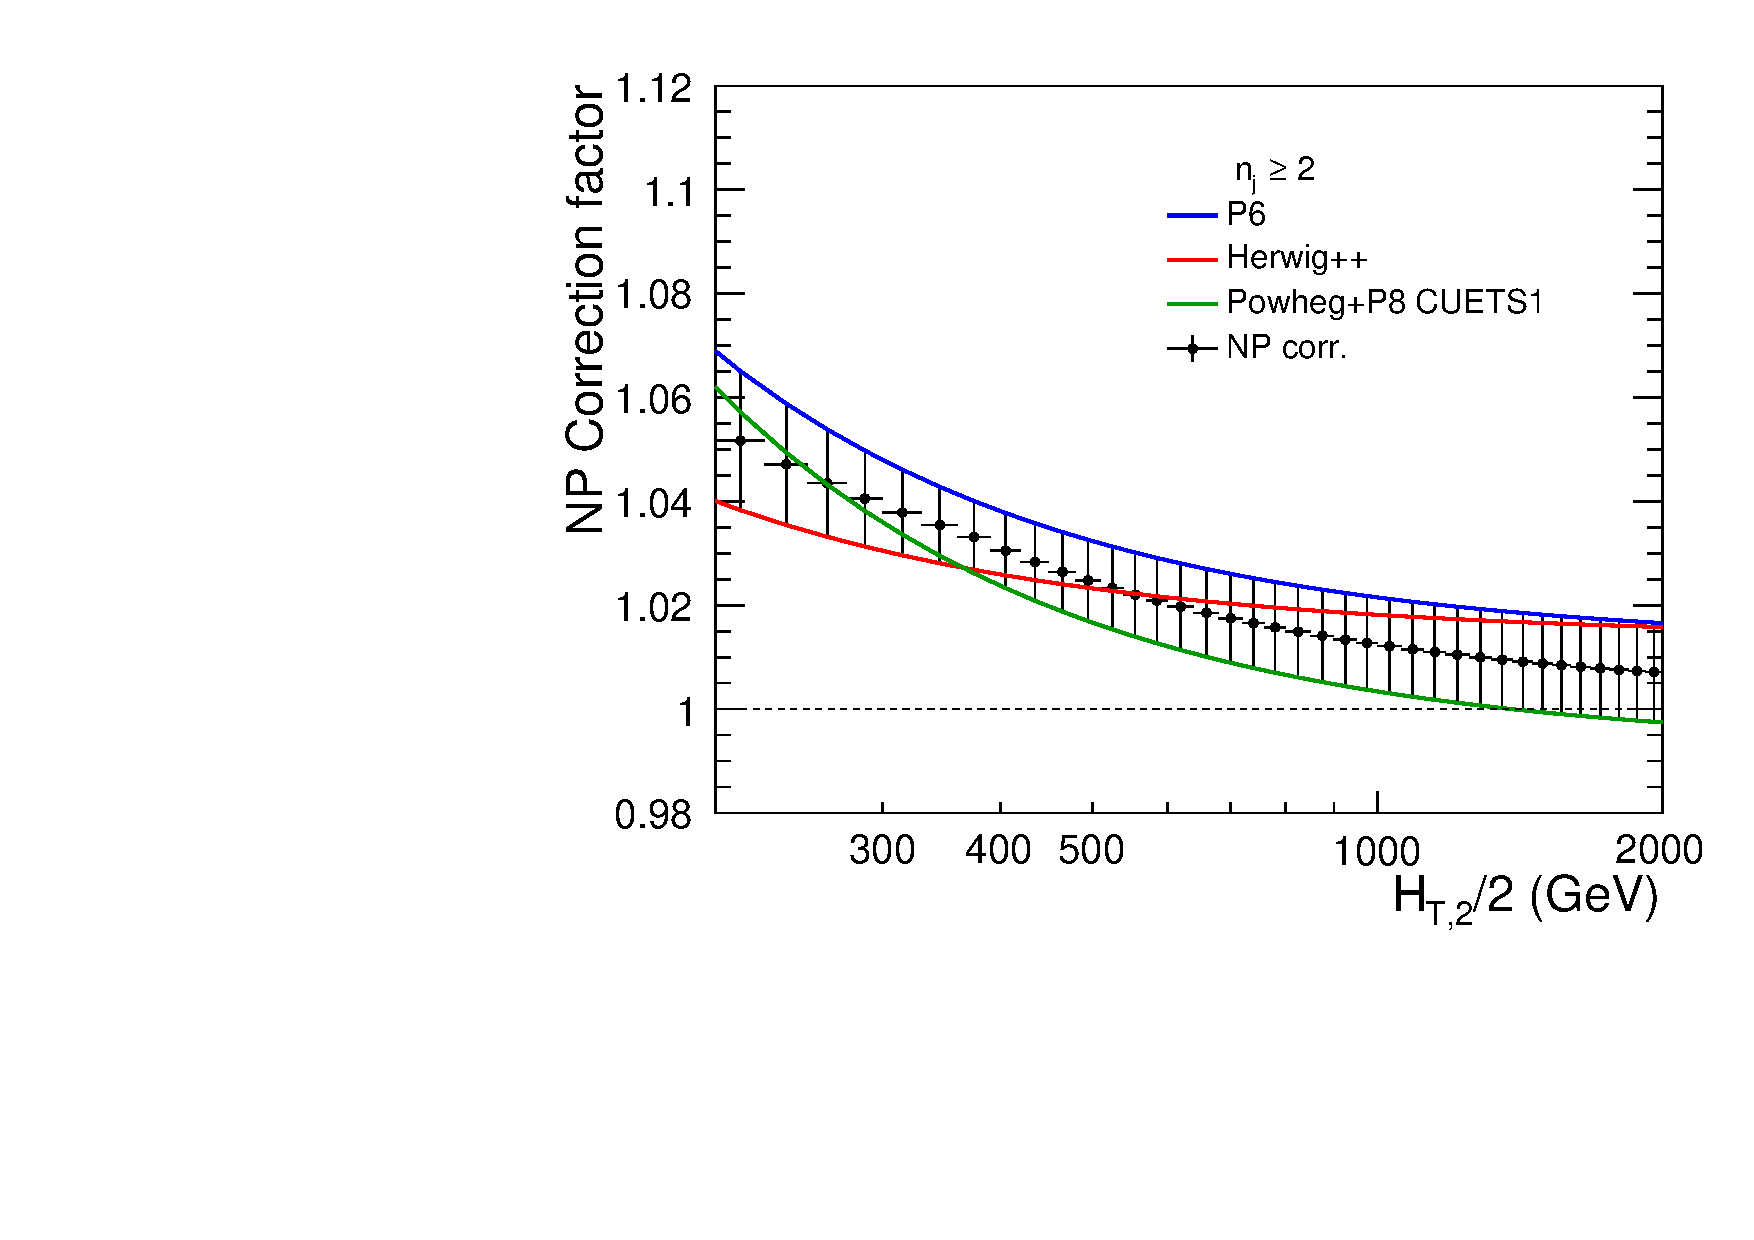
\includegraphics[width=0.51\textwidth]{Plots_HT_2_150/Final_NP_Corr_2.pdf}%
 ~~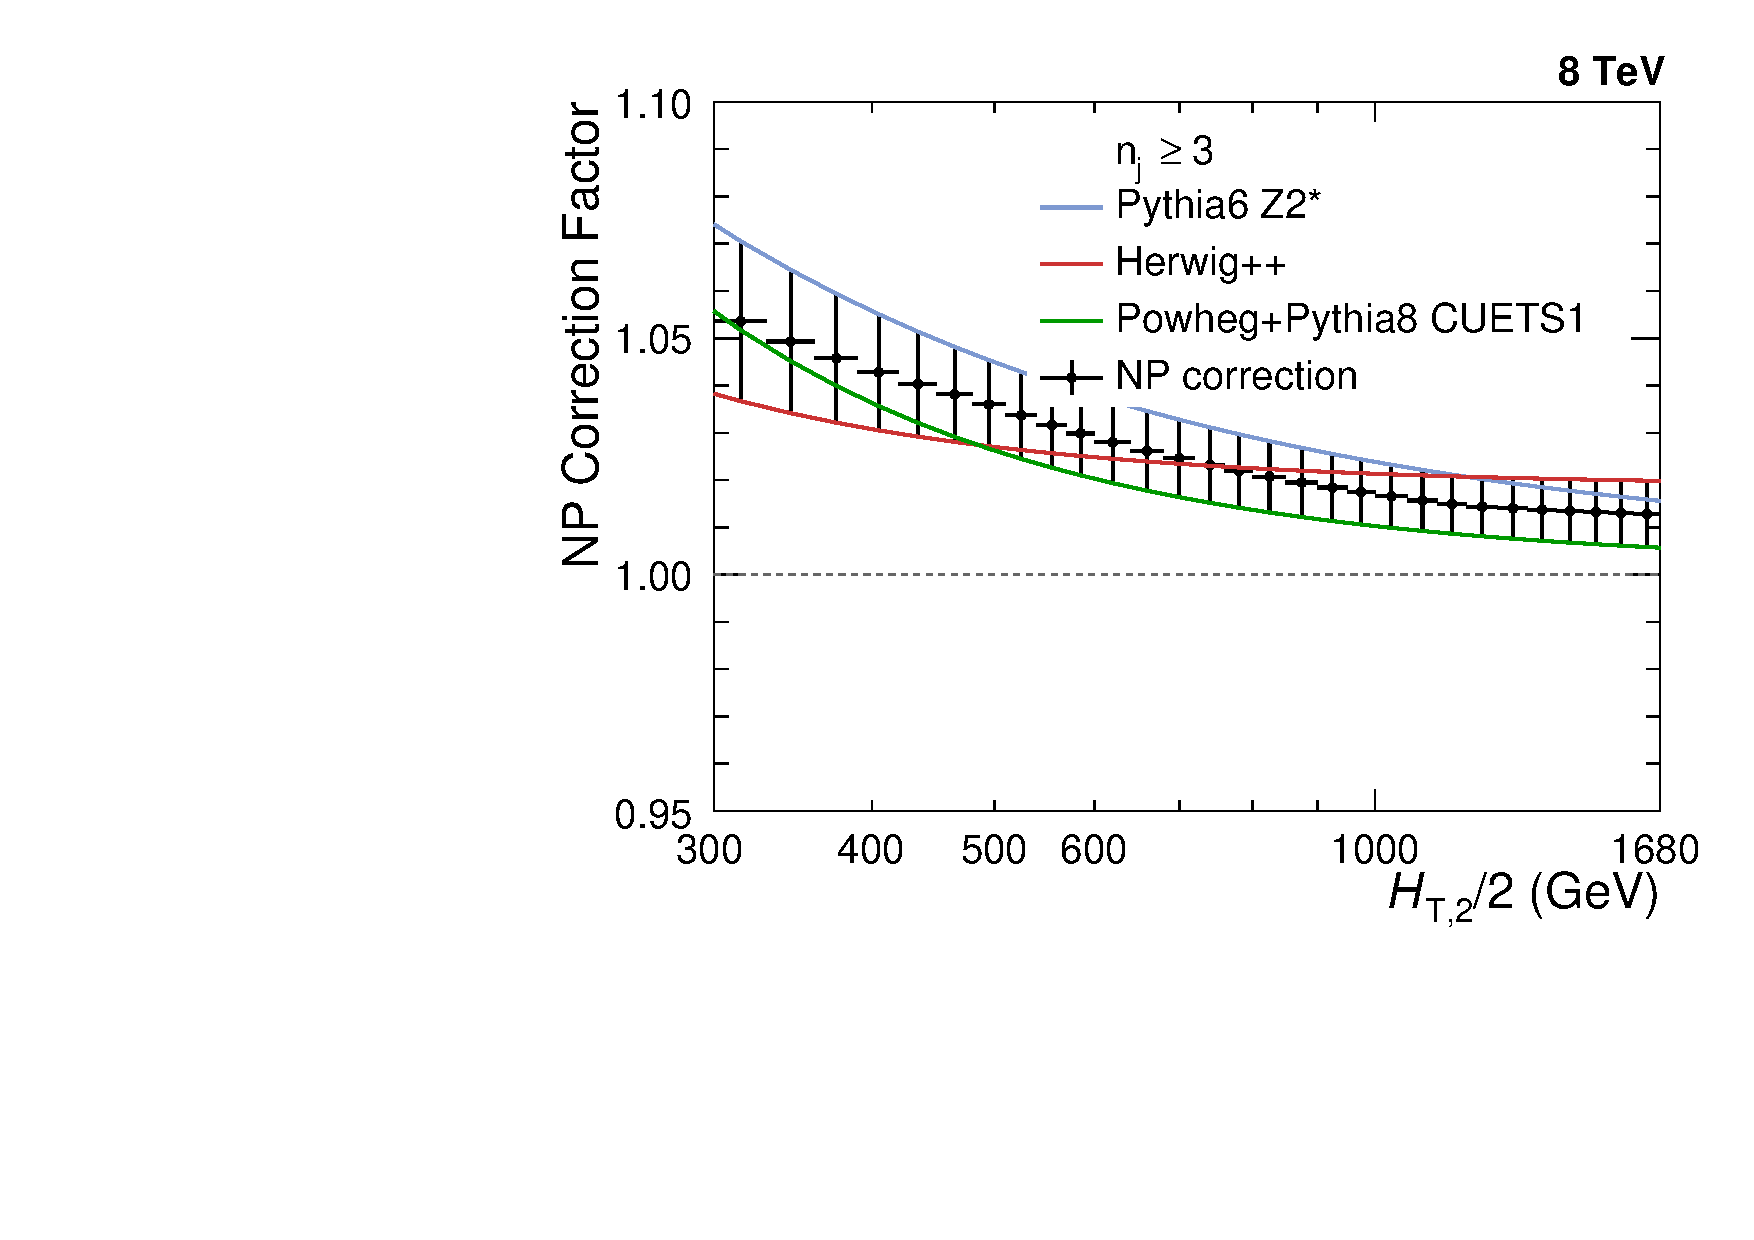
\includegraphics[width=0.51\textwidth]{Plots_HT_2_150/Final_NP_Corr_3.pdf}\\
 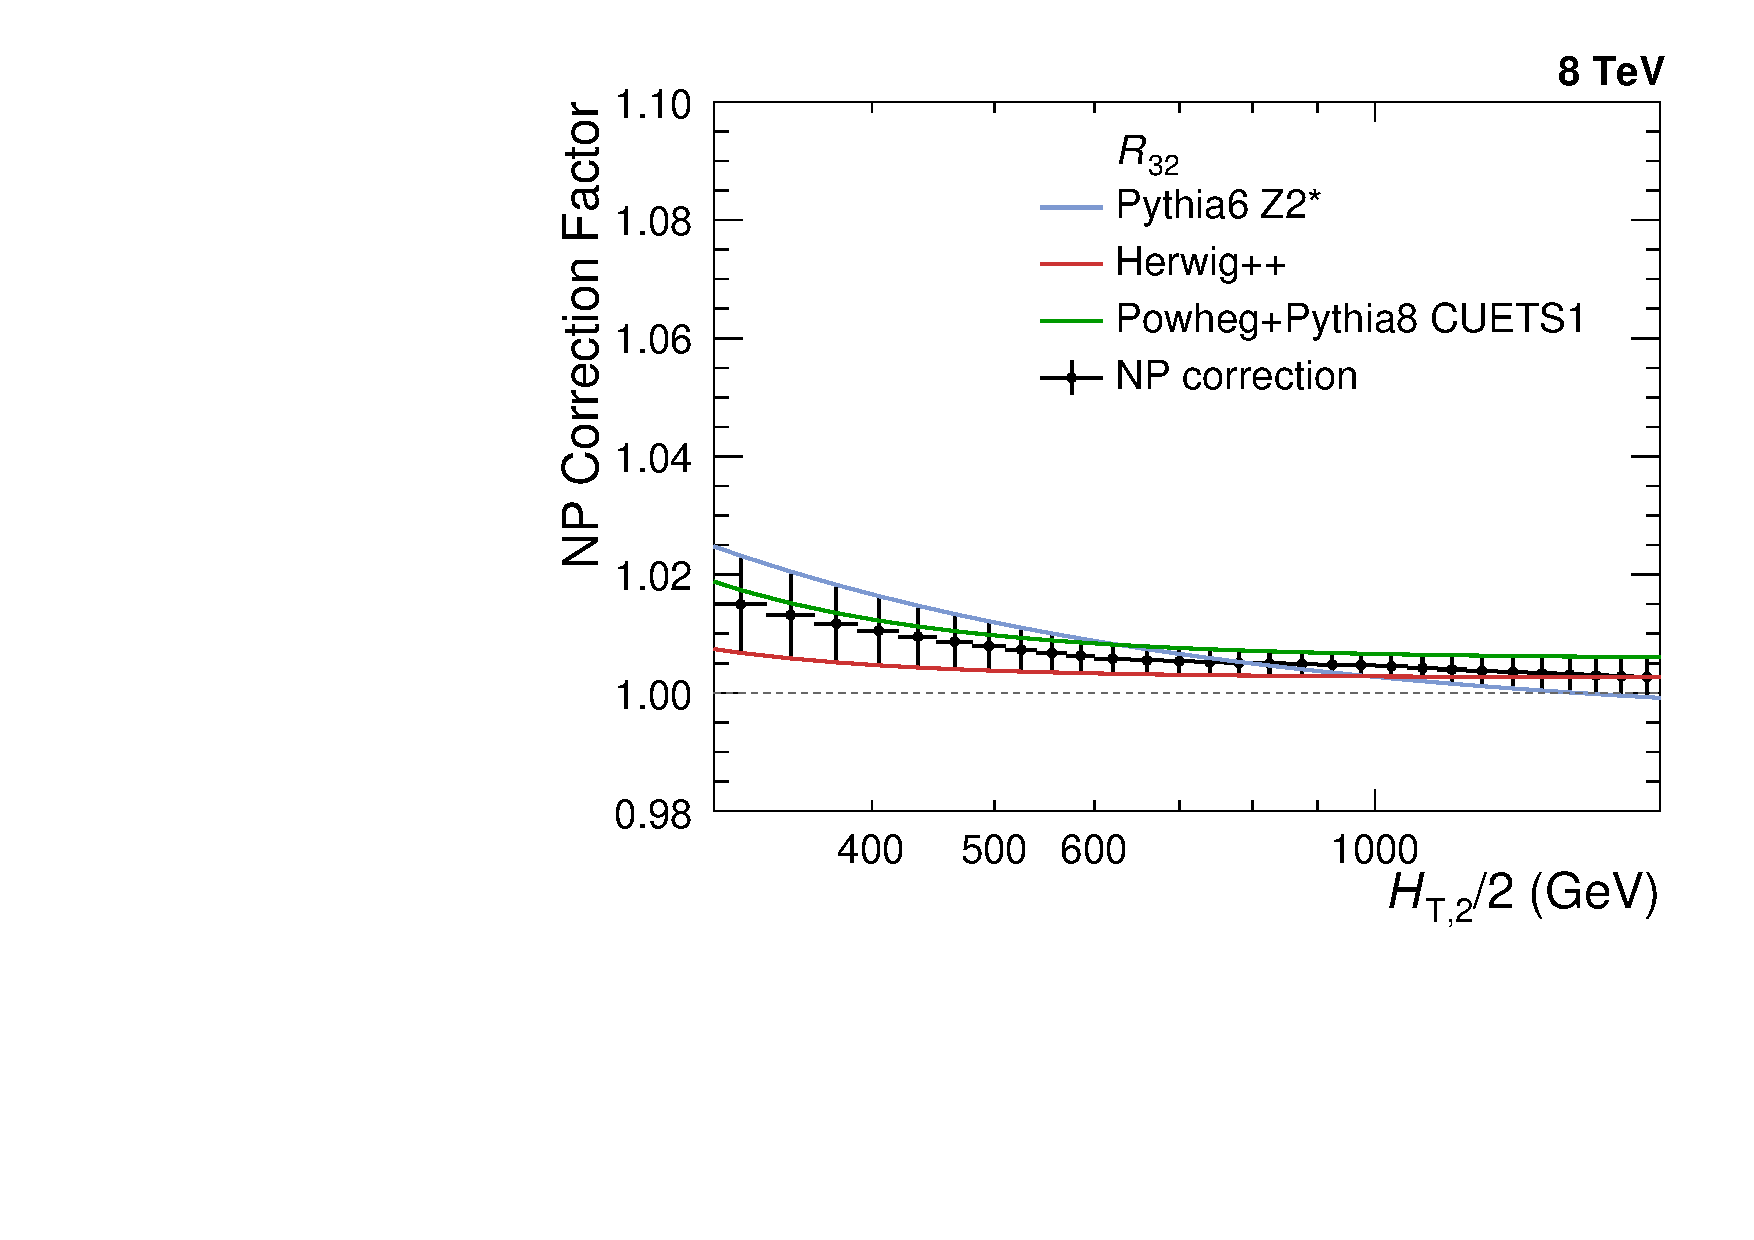
\includegraphics[width=0.51\textwidth]{Plots_HT_2_150/Final_NP_Corr_Ratio_32.pdf}
 \caption{Fits to the nonperturbative corrections obtained for inclusive 2-jet (top left) and 3-jet (top right) event cross sections, as well as ratio \ratio, as a function of \httwo for $|y|<2.5$.}
 \label{fig:np_factors}
 \end{center}
\end{figure}
\begin{comment}
\subsection{Electroweak corrections (EWK)}
\label{sec:EWK}

The NLO theory calculations are corrected for electroweak effects. The quark-quark scattering processes like qq̄ → qq̄, q i q̄ i → q j q̄ j or q i q̄ 0 i → q j q̄ 0 j can be mediated through exchange of photon (γ) or vector boson (V) at LO. At NLO the quark propagators and qq̄g vertex gets 1-loop correction from V exchange. All these processes contributes to the multijet production final states, called electro-weak (EWK) corrections, which are calculated in Ref.[58]. The distribution of EWK correction factors are shown as a function of jet p T and |y| in Figure 6.1. The figure shows that EWK correction factors
are mostly important in the central |y| regions where the correction factor can go upto 14\%. In the outer rapidity regions, the effect of EWK correction is small and is ∼ 2\%. It is to be noticed that on the outer regions, it mainly decreses the value of cross-sections while in the central rapidity regions it enhances the cross-section for most regions of phase-space


The fixed-order QCD calculations do not include contributions arising from virtual
exchanges of massive W and Z bosons. The electroweak corrections (EWK) are calculated by ~\cite{Dittmaier:2012kx} and are
applied as a bin-by-bin correction factor to the fixed-order calculation of \NLOJETPP 
as well as the MC predictions of \MadGraphF \plus \PYTHIAS. The correction factors in the
phase space of the measurement are given in Figure~\ref{fig:EW} for inclusive 2-jet events. 
For inclusive 3-jet events are not calculated yet. The EWK increases up to 5\% for \httwo $>$ 1 TeV and significantly improves the
agreement between data and prediction. Since the guess from theory side is that EWK for inclusive 2-jet and 3-jet will be similar, so for \ratio, it is assumed to be equal to the factor of 1.

\begin{figure}[!htbp]
\begin{center}
  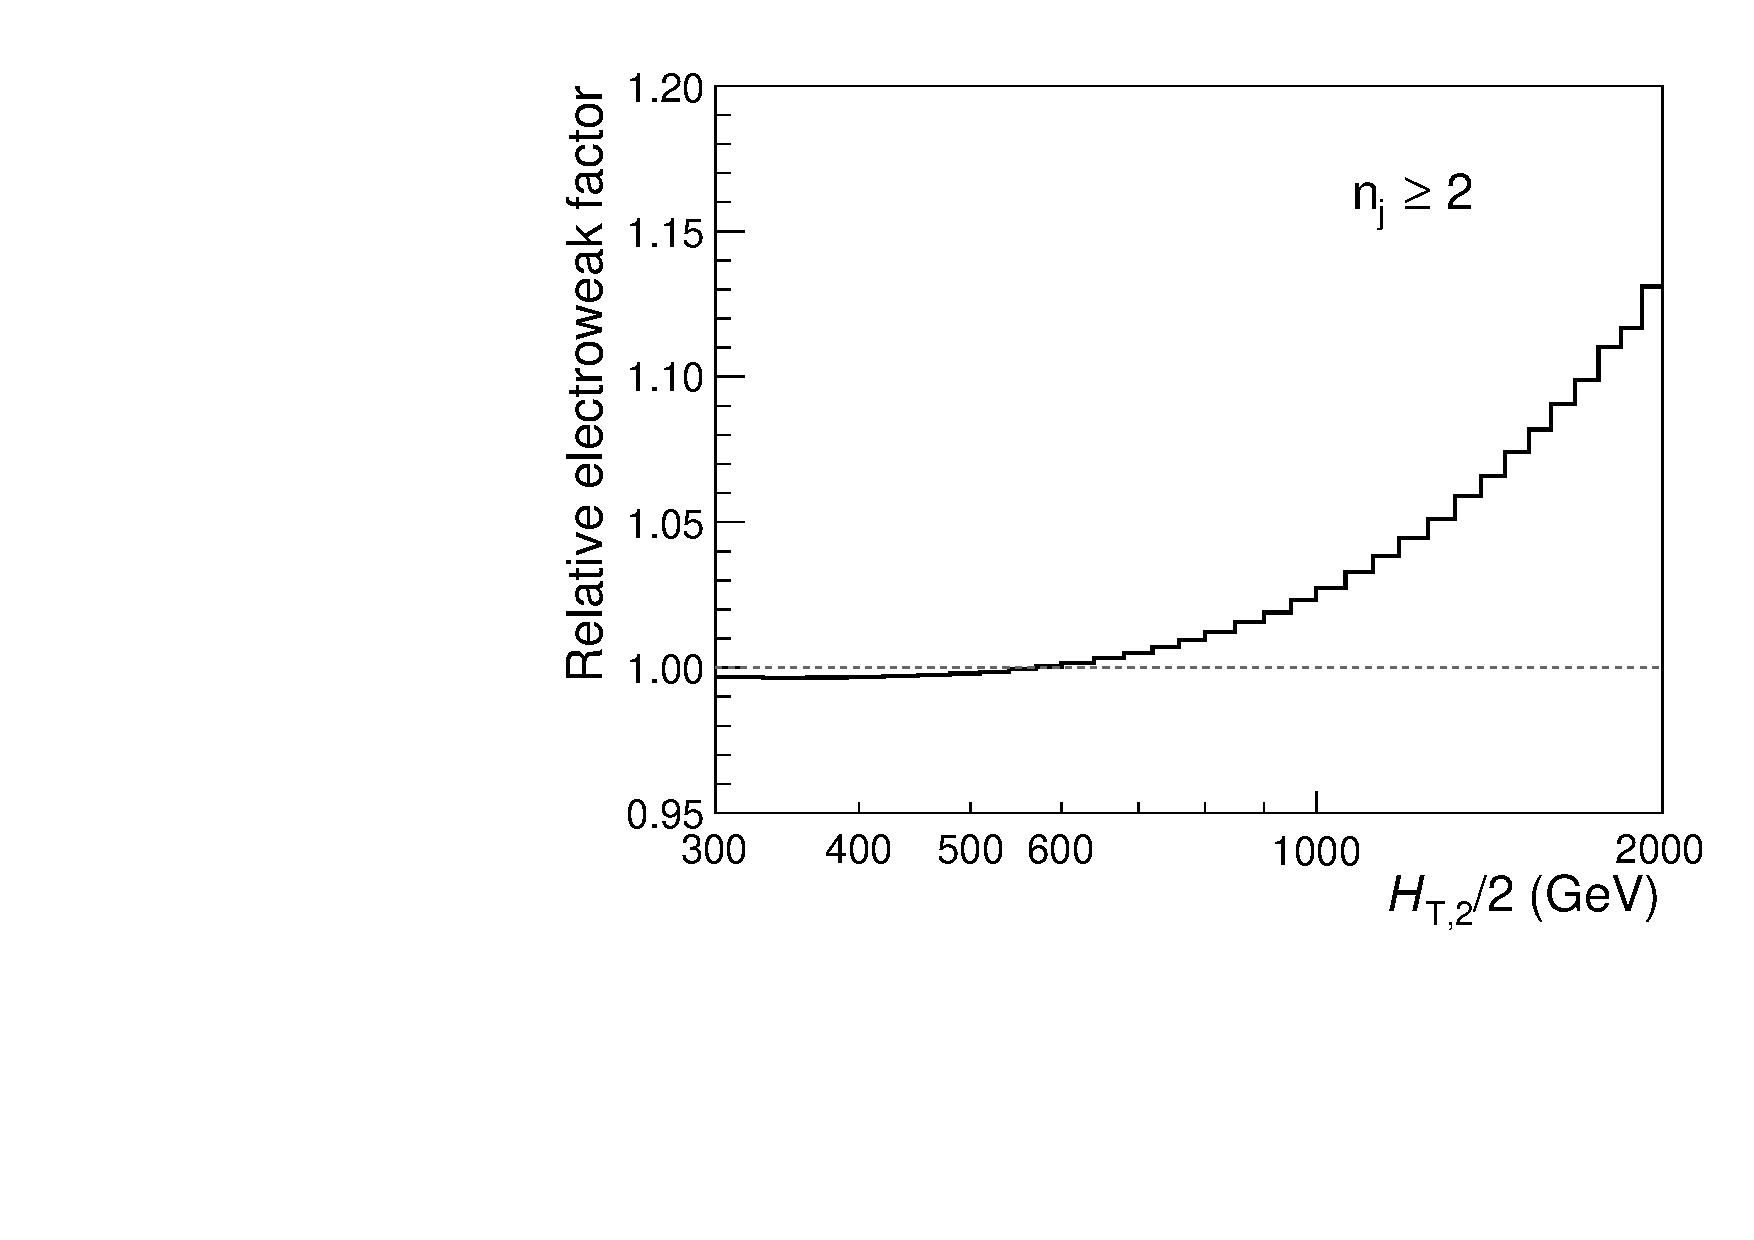
\includegraphics[width=0.5\textwidth]{Plots_HT_2_150/EW_2.pdf}
  \caption{The electroweak corrections for inclusive 2-jet as a function of \httwo.}
  \label{fig:EW}
\end{center}
\end{figure}

\subsection{Theory uncertainties}
In this subsection, the derivation of theoretical uncertainties from various 
sources have been described. The total systematic theoretical uncertainties
are evaluated as the quadratic sum of the scale, PDF, and NP uncertainties, and are tabulated in the table~\ref{tab:theory_unc}. 
Figure~\ref{fig:theory_unc} gives the overview of systematic theoretical 
uncertainties affecting the cross section measurement
for inclusive 2-jet (top left) and 3-jet events (top right) and their
ratio \ratio (bottom), using CT10 PDF 
set. The uncertainties on non-perturbative 
corrections have been already presented together
with the obtained correction factors in Section~\ref{sec:NPcorr}. 

The computation of the NLO predictions with \NLOJETPP is also subject
to statistical fluctuations from the complex numerical integrations.
For the inclusive 2-jet event cross sections this uncertainty is
smaller than about a per mille, while for the inclusive 3-jet event
cross section it amounts to 1--9 per mille.

Higher orders of electroweak origin affect jet cross sections at large
jet \pt. These electroweak corrections (EWK) have been calculated for
the inclusive 1-jet and 2-jet case, cf.\ Ref.~\cite{Dittmaier:2012kx},
but are not yet known for 3-jet production. Therefore, they are
considered for the 2-jet events, while for the 3-jet event cross
section and for the ratio they have been neglected.

\begin{figure}[!htbp]
\begin{center}
  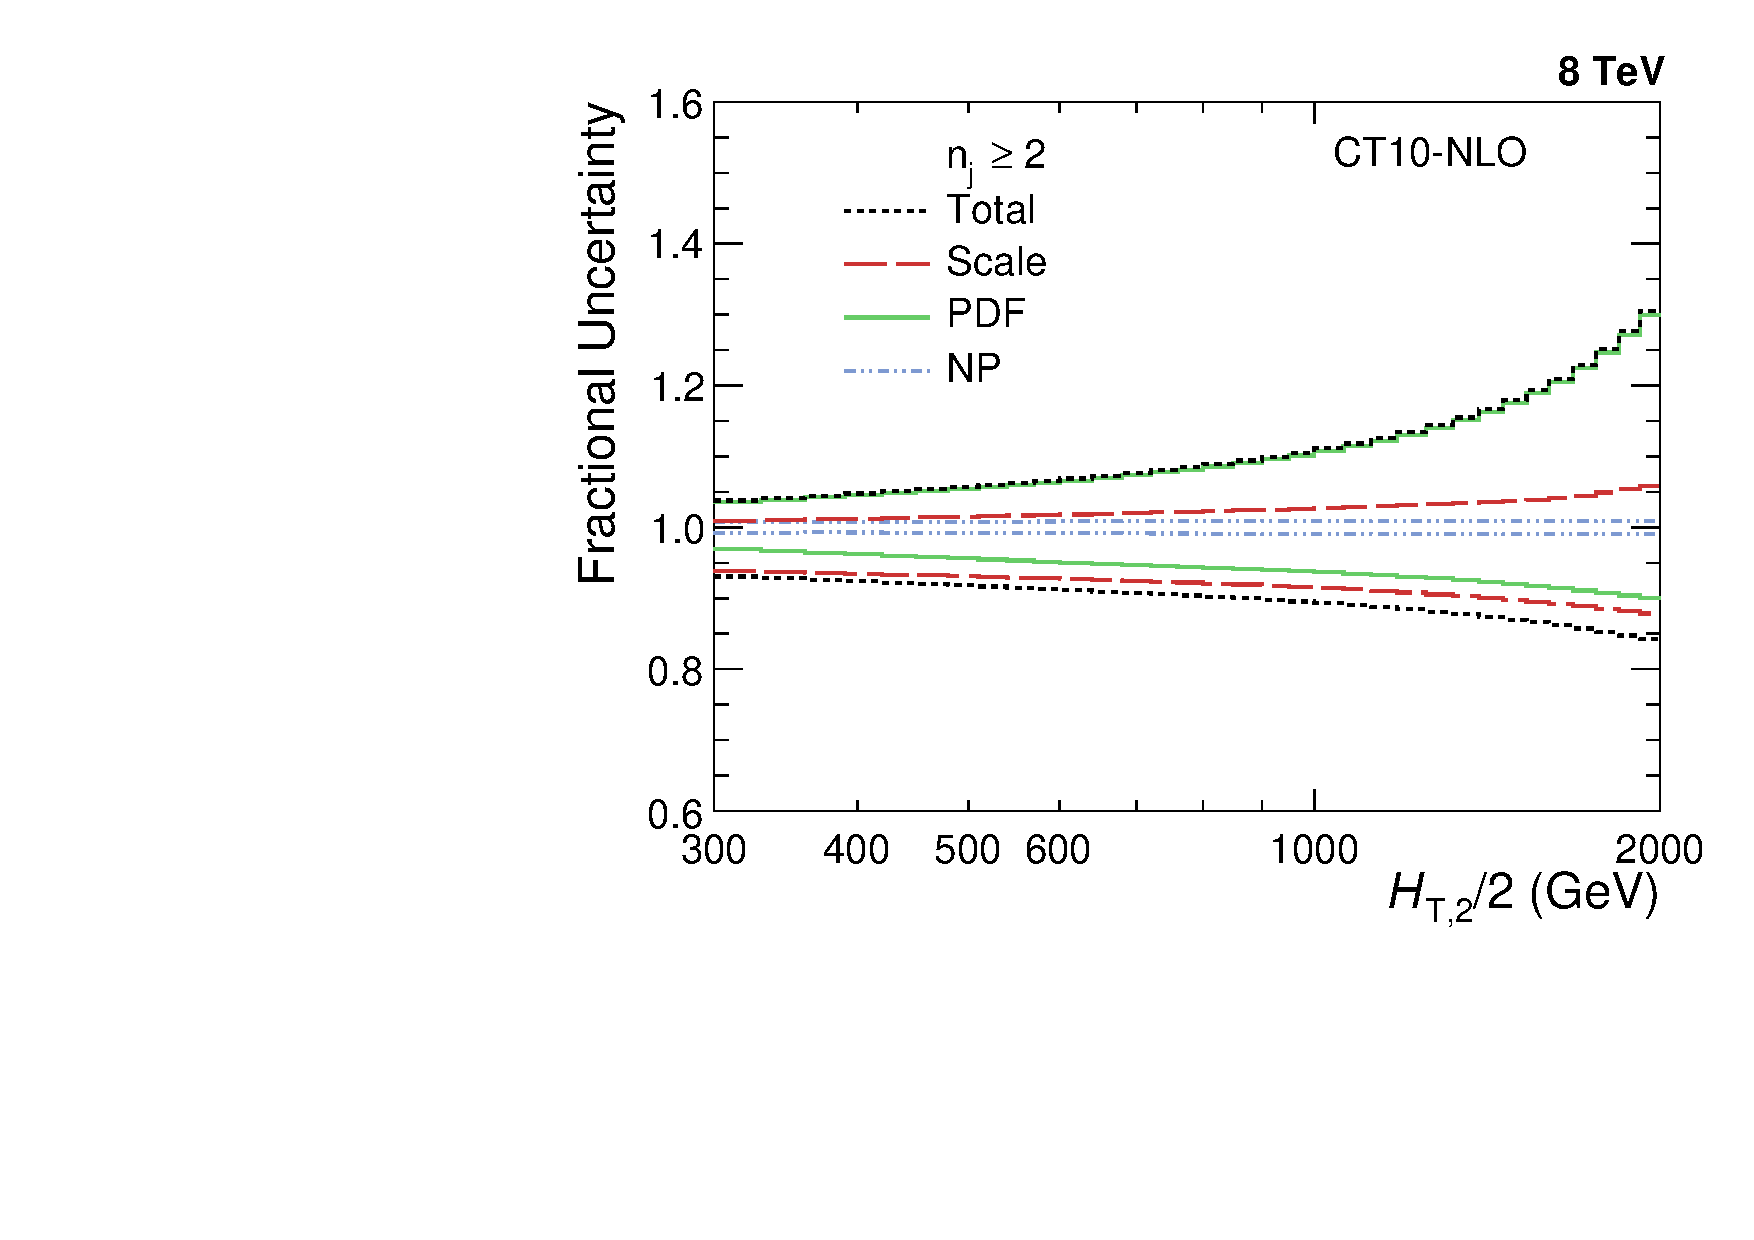
\includegraphics[width=0.5\textwidth]{Plots_HT_2_150/Theory_Unc_2.pdf}%
  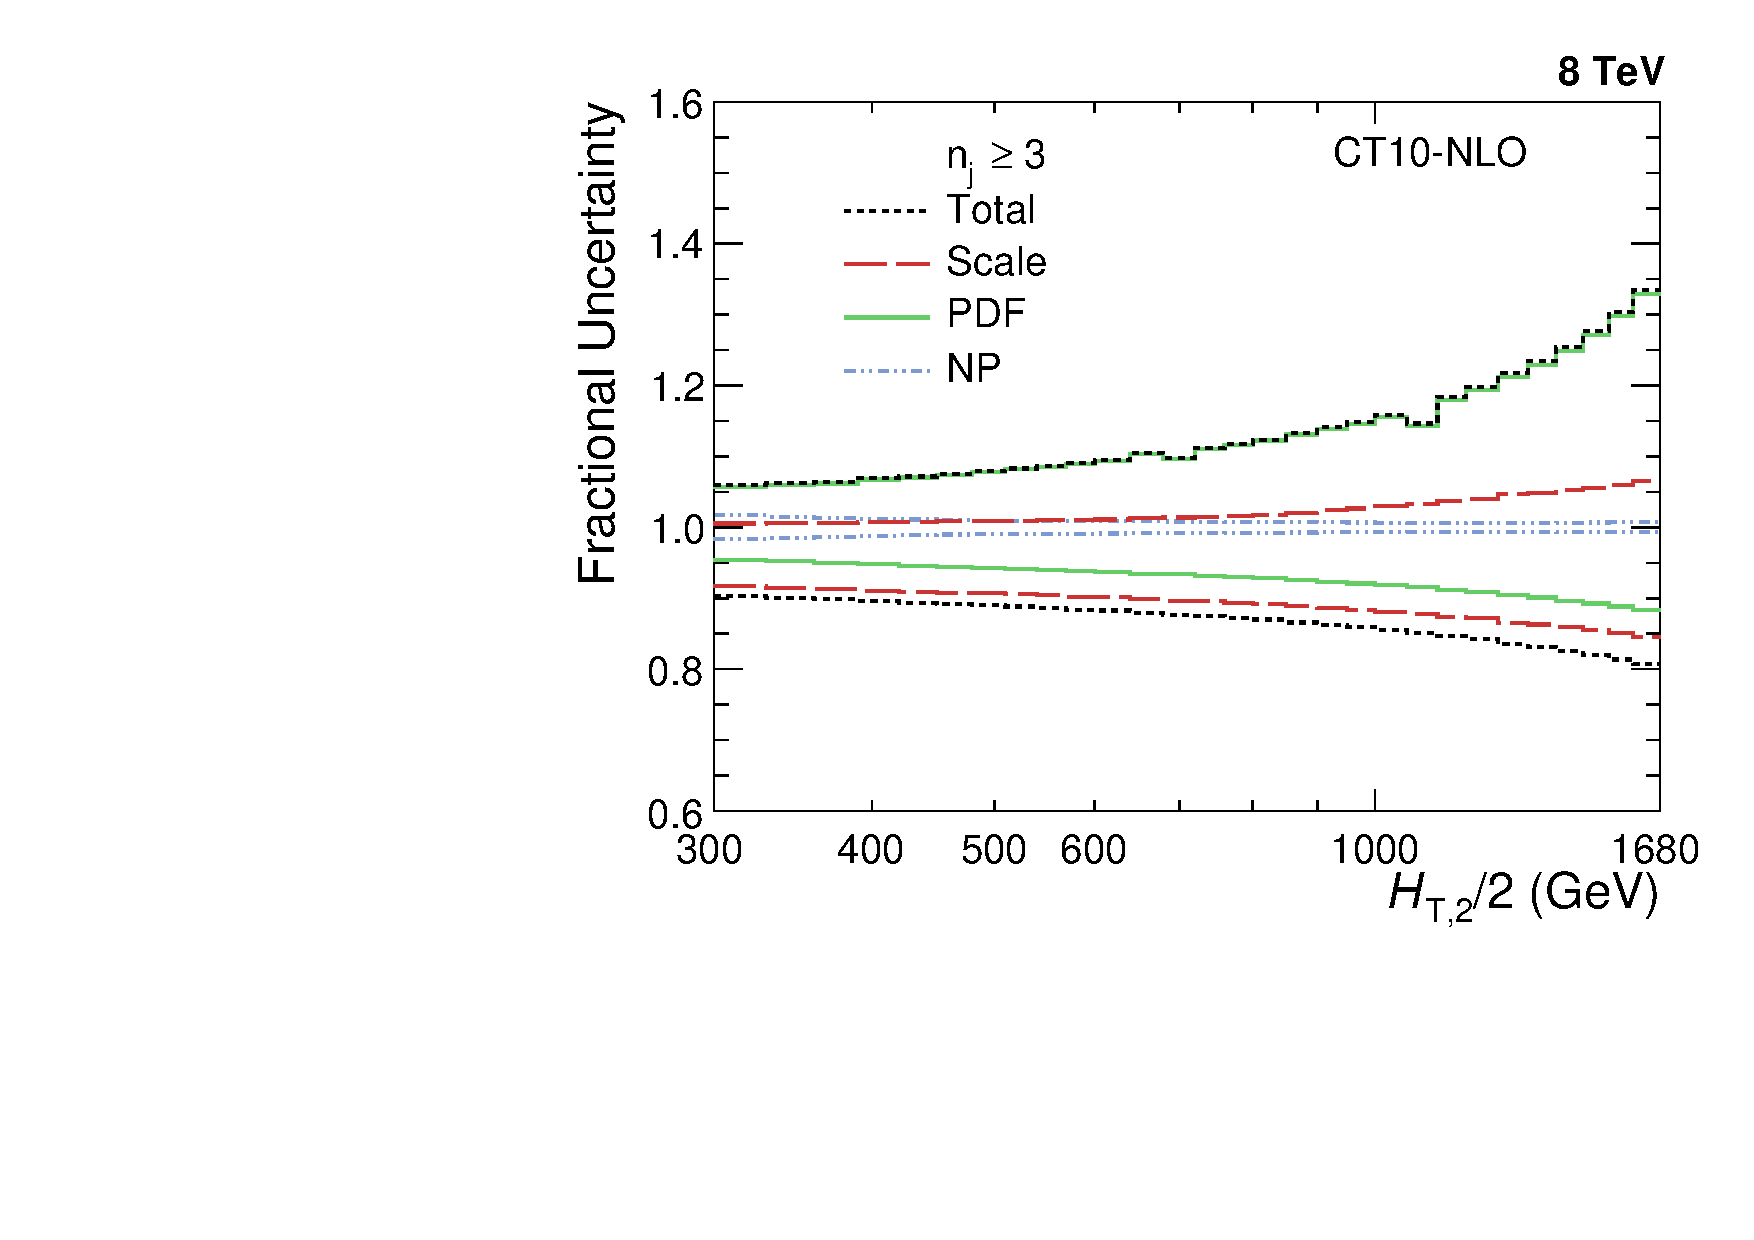
\includegraphics[width=0.5\textwidth]{Plots_HT_2_150/Theory_Unc_3.pdf}\\
  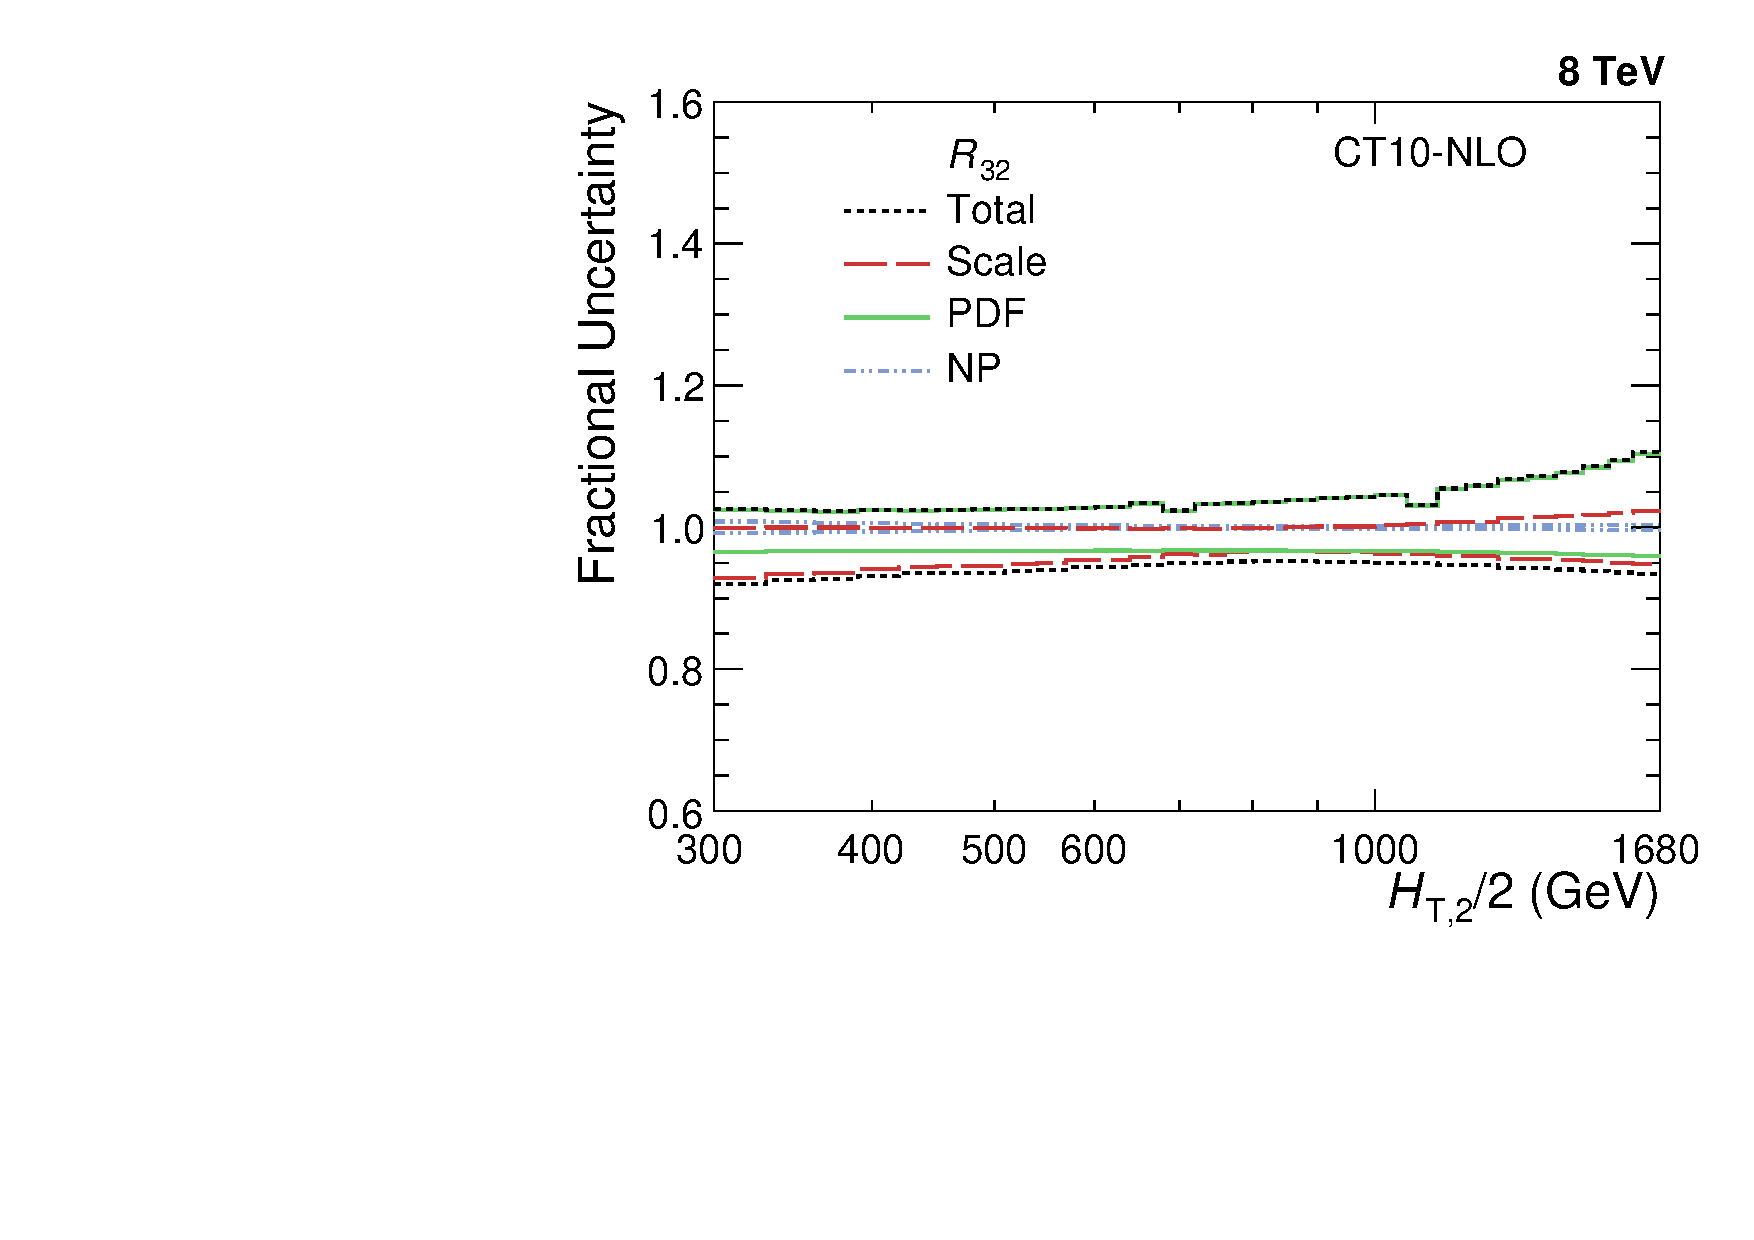
\includegraphics[width=0.5\textwidth]{Plots_HT_2_150/Theory_Unc_Ratio_32.pdf}\\  
  \caption{Overview of systematic theoretical uncertainties affecting the cross section measurement
    for inclusive 2-jet (top left) and 3-jet events (top right) and their ratio \ratio (bottom)
    using CT10 PDF set. The total uncertainty is calculated
    by adding in quadrature the individual sources of uncertainty.}
  \label{fig:theory_unc}
\end{center}
\end{figure}


\begin{table}[!htbp]
  \caption{Overview of systematic theoretical uncertainties affecting the cross section measurement
    for inclusive 2-jet and 3-jet events using CT10 PDF set. }
  \label{tab:theory_unc}
  \centering
  \vspace{2mm}
  \begin{tabular}{cccc}
    \hline\hline
    Uncertainty Source & {\bf Inclusive 2-jet} & {\bf Inclusive 3-jet} & {\bf \ratio} \rbthm\\ \hline
    {\bf \textcolor{red} {Scale}} & 5 to 13\% & 11 to 17\% & 6 to 8\% \rbtrr\\
    {\bf \textcolor{green!50!white} {PDF}} & 2 to 30\% & 5 to 50\% & 2 to 7\% \rbtrr\\
    {\bf \textcolor{blue} {NP}} & 1\% & 1 to 2\%  & $<$ 1\% \rbtrr\\
    \hline\hline
  \end{tabular}
\end{table}

\subsubsection{Scale uncertainties}
The uncertainty related to unknown higher orders of the perturbative
series is evaluated with the conventional recipe of varying the
default scale \httwo chosen for \mur and \muf independently in the
following six combinations: (\mur/\httwo, \muf/\httwo) = (1/2,1/2),
(1/2,1), (1,1/2), (1,2), (2,1) and (2,2). The maximal upwards and
downwards deviations in cross section from the central prediction are
taken as scale uncertainty. This uncertainty ranges for inclusive
2-jet events from 5\% to 13\%, for inclusive 3-jet events from 11\%
to 17\% and \ratio from 6\% to 8\%.

\subsubsection{PDF uncertainties}
PDF uncertainties are evaluated according to the prescriptions given
for each PDF set. Uncertainties on \alpsmz are not considered, since
this value is later on determined from a fit to the data. The PDF
uncertainty as derived with the CT10 PDF set ranges from 2\% to 30\%
for inclusive 2-jet events and from 5\% to 50\% for inclusive 3-jet
events and from 2\% to 7\% for \ratio.

\section{Comparison of theory to data}

Figure~\ref{fig:data_NL0_MC} shows the measured inclusive 2-jet and
3-jet event cross sections as a function of \httwo after unfolding for
detector effects. On the left, the measurements are compared to the
\NLOJETPP predictions using the CT10 PDF set, corrected for NP effects
and in addition for EWK effects in the 2-jet case.  On the right, the
comparison is made to the predictions from \MadGraphF + \PYTHIAS with
tune \Ztwostar, corrected for EWK effects in the 2-jet case. On a
logarithmic scale, the data are in agreement with the NLO predictions
over the whole range of \httwo from 300\GeV up to 2.0 (2-jet) and 1.68\TeV (3-jet) respectively.

\begin{figure}[!htbp]
  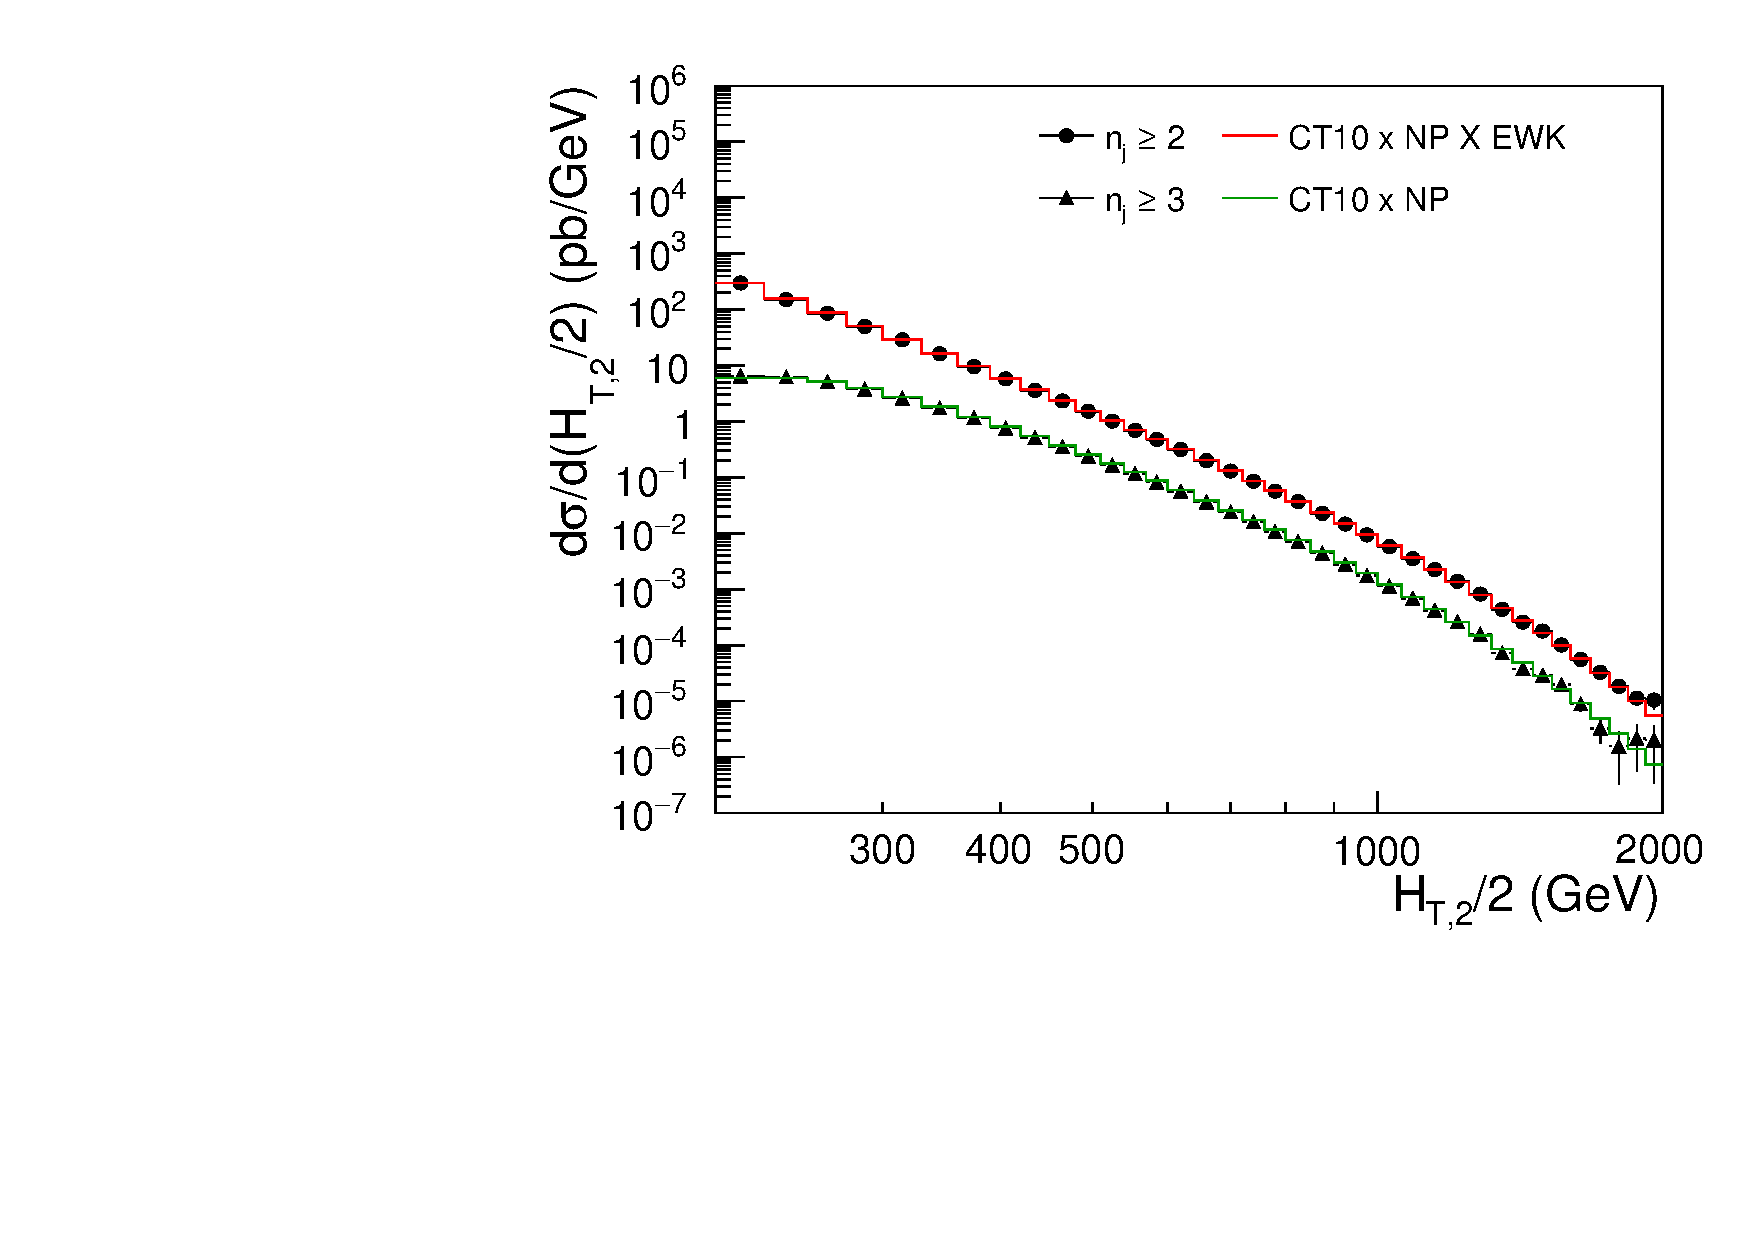
\includegraphics[width=0.50\textwidth]{Plots_HT_2_150/Comparison_data_theory_EWK.pdf}%
  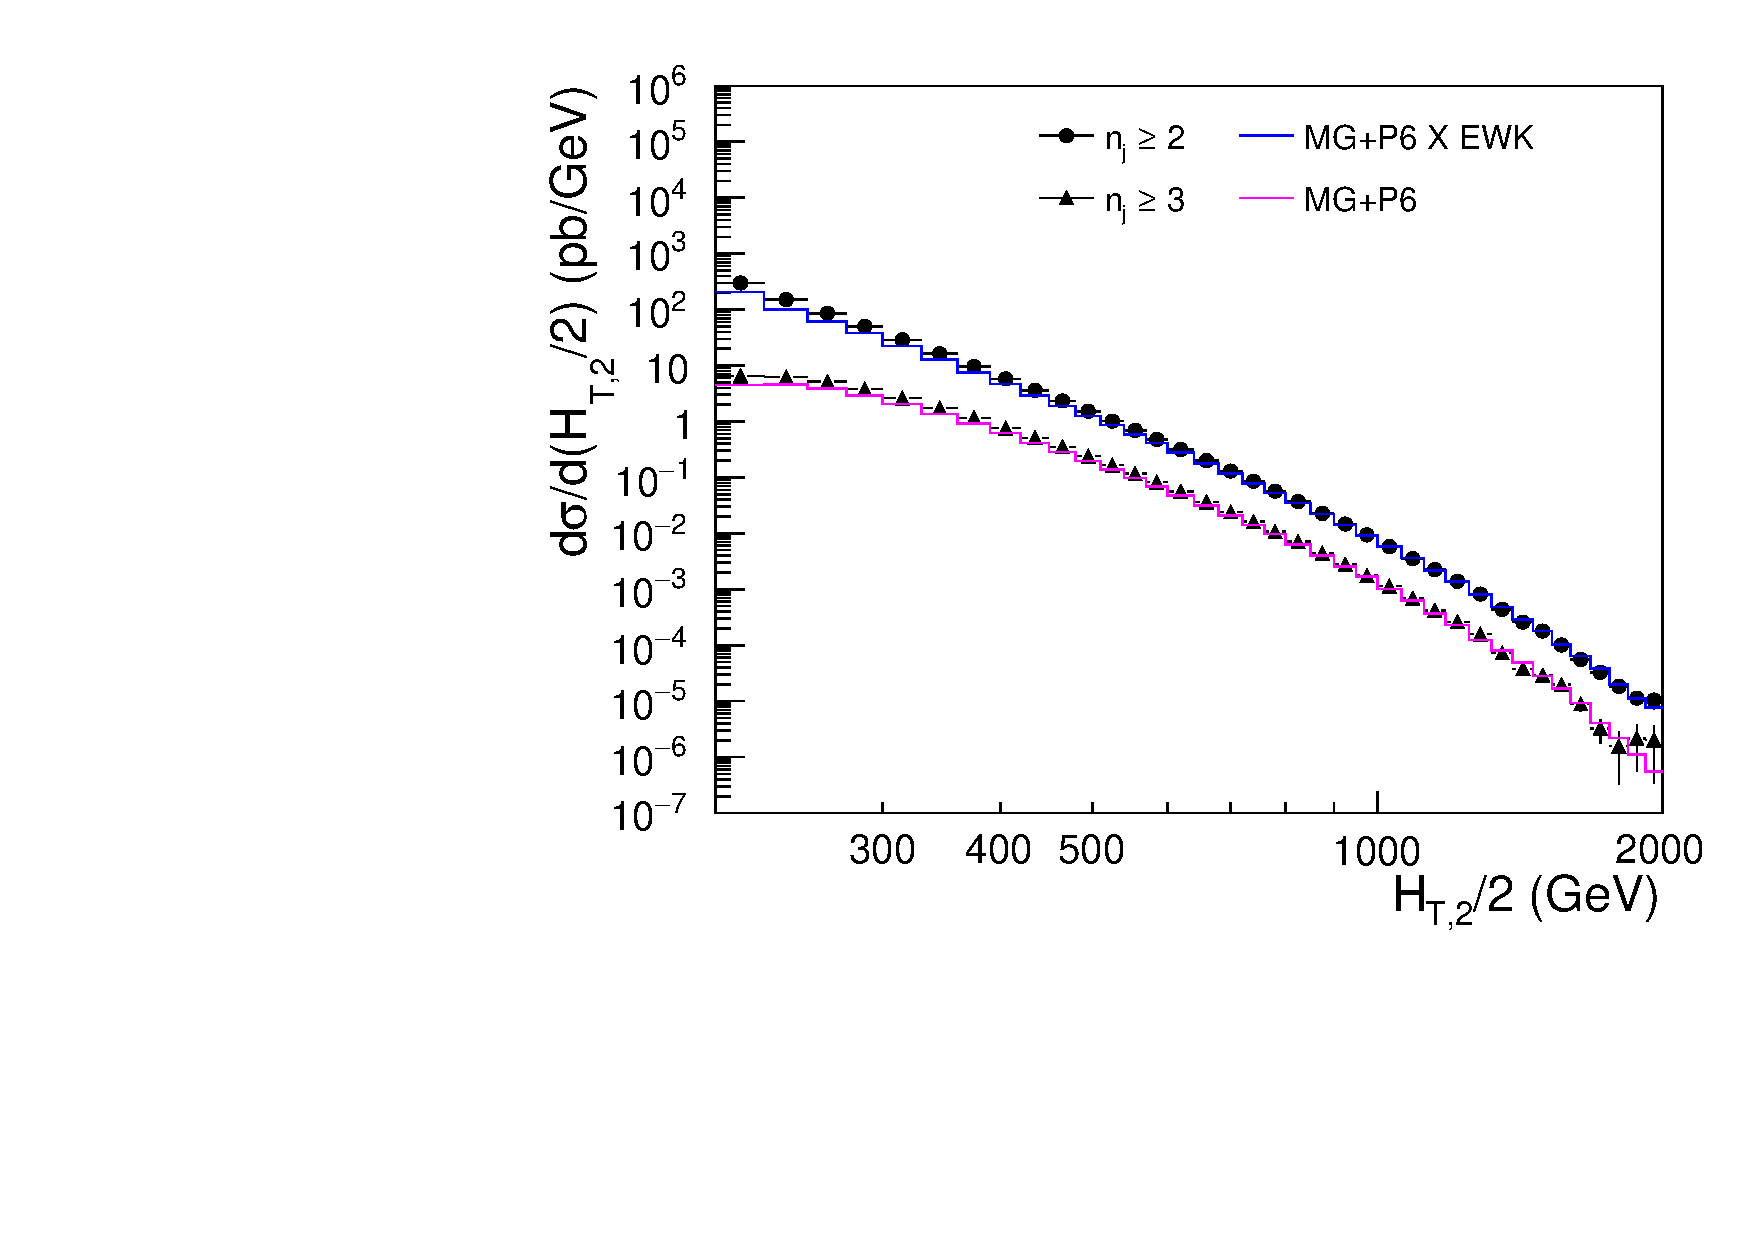
\includegraphics[width=0.50\textwidth]{Plots_HT_2_150/Comparison_data_MC_EWK.pdf}\\
  \caption{Comparison of the inclusive 2-jet and 3-jet event cross
    sections as a function of \httwo to theoretical predictions. On
    the (left), the data (points) are shown together with
    \NLOJETPP predictions (line) using the CT10 PDF set, corrected for
    NP and EWK (2-jet) or only NP effects (3-jet).  On the
    (right), the data (points) are compared to predictions from
    \MadGraphF + \PYTHIAS with tune \Ztwostar (line), corrected for
    EWK effects in the 2-jet case. The error bars correspond to the
    total uncertainty, for which the statistical and systematic
    uncertainties are added in quadrature.}
  \label{fig:data_NL0_MC}
\end{figure}

For better visibility the ratios of data over the \NLOJETPP
predictions using the CT10 PDF set are shown in
Figure~\ref{fig:data_NLOPdfs}. The data are well described by the
predictions within their uncertainty, which is dominated at large
\httwo by PDF effects in the upwards and by scale variations in the
downwards direction. A trend towards an increasing systematic excess
of the 2-jet data with respect to theory, starting at about 1\TeV in
\httwo, is remedied by the inclusion of EWK corrections. In the 3-jet
case the statistical precision of the data and the reach in \httwo is
insufficient to observe any effect. The alternative PDF sets MSTW2008
and NNPDF2.3 exhibit a small underestimation of the cross sections at
high \httwo.

\begin{figure}[!htbp]
\begin{center}
  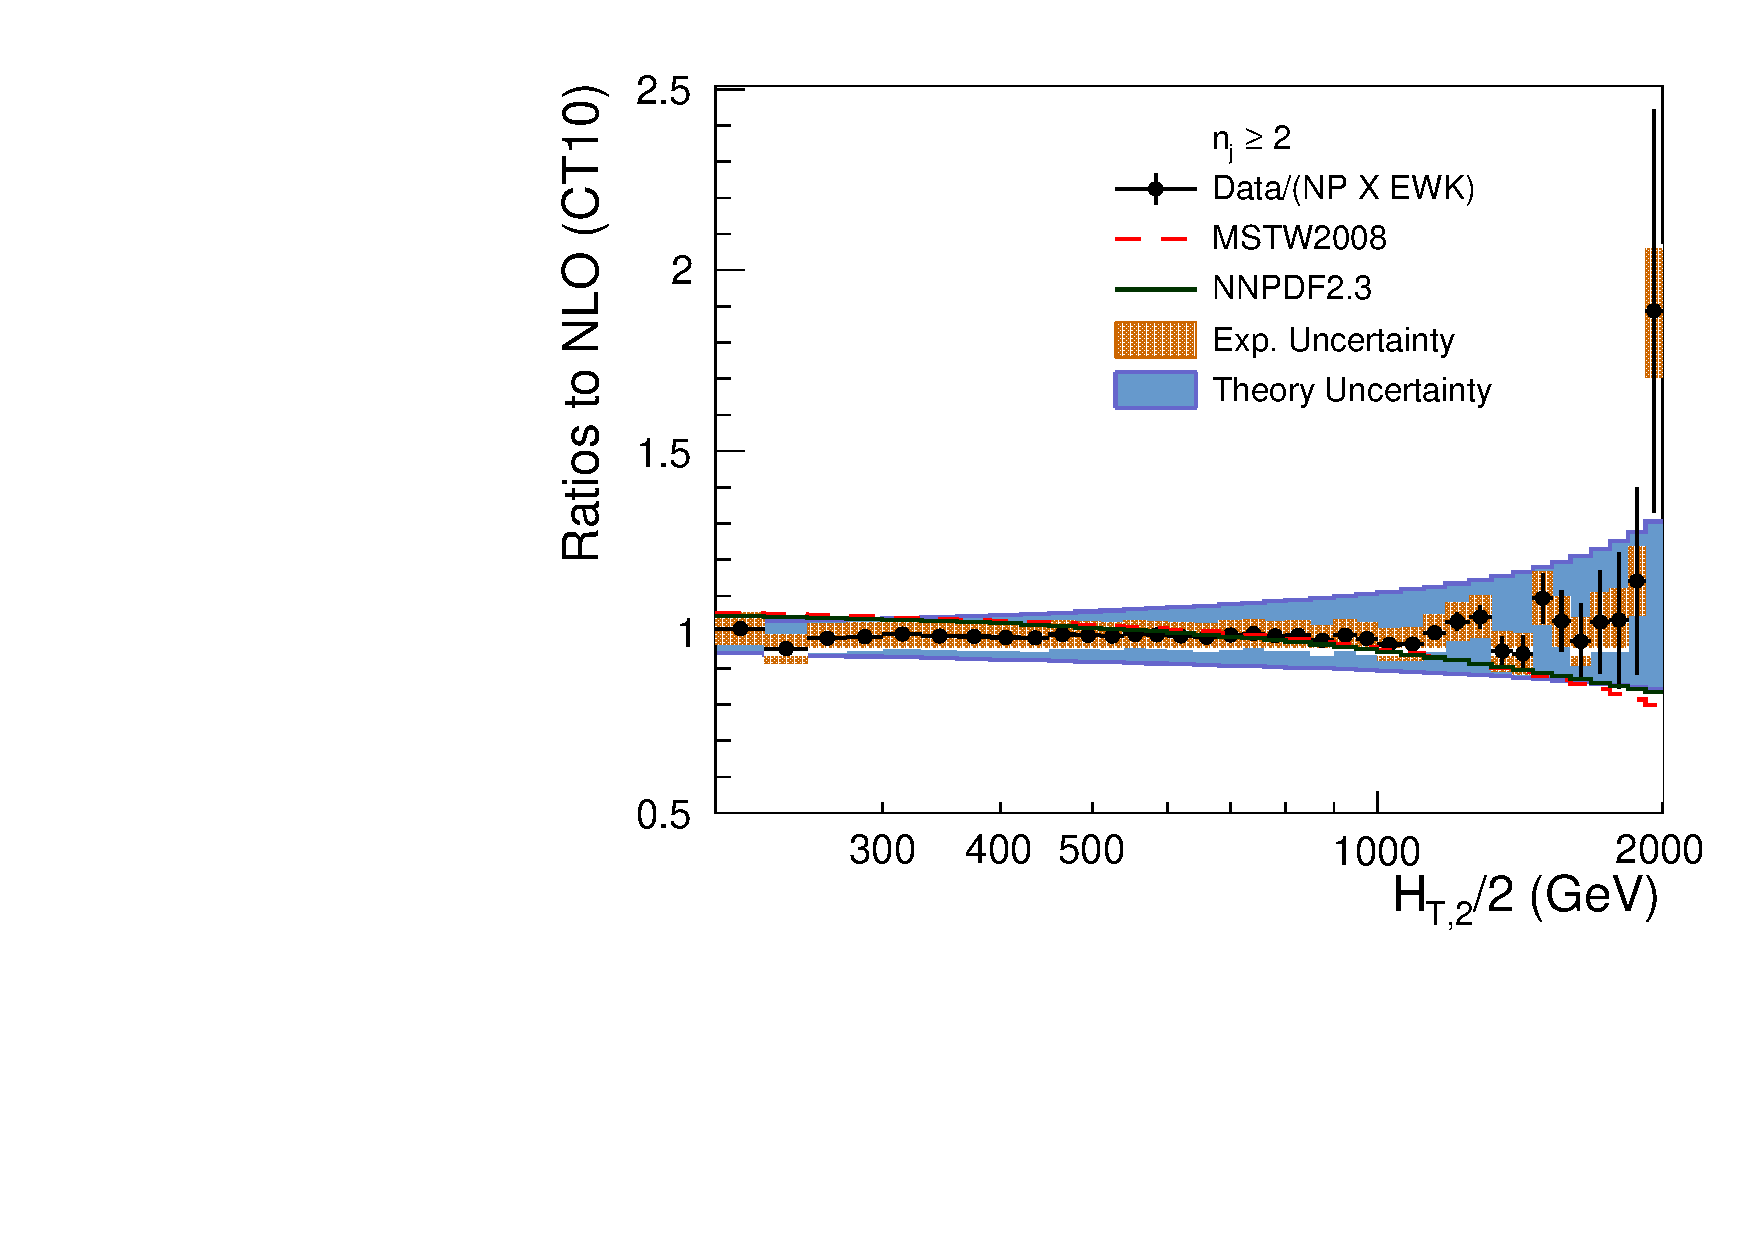
\includegraphics[width=0.5\textwidth]{Plots_HT_2_150/Comparison_data_NLO_Pdfs_2_EWK.pdf}%
  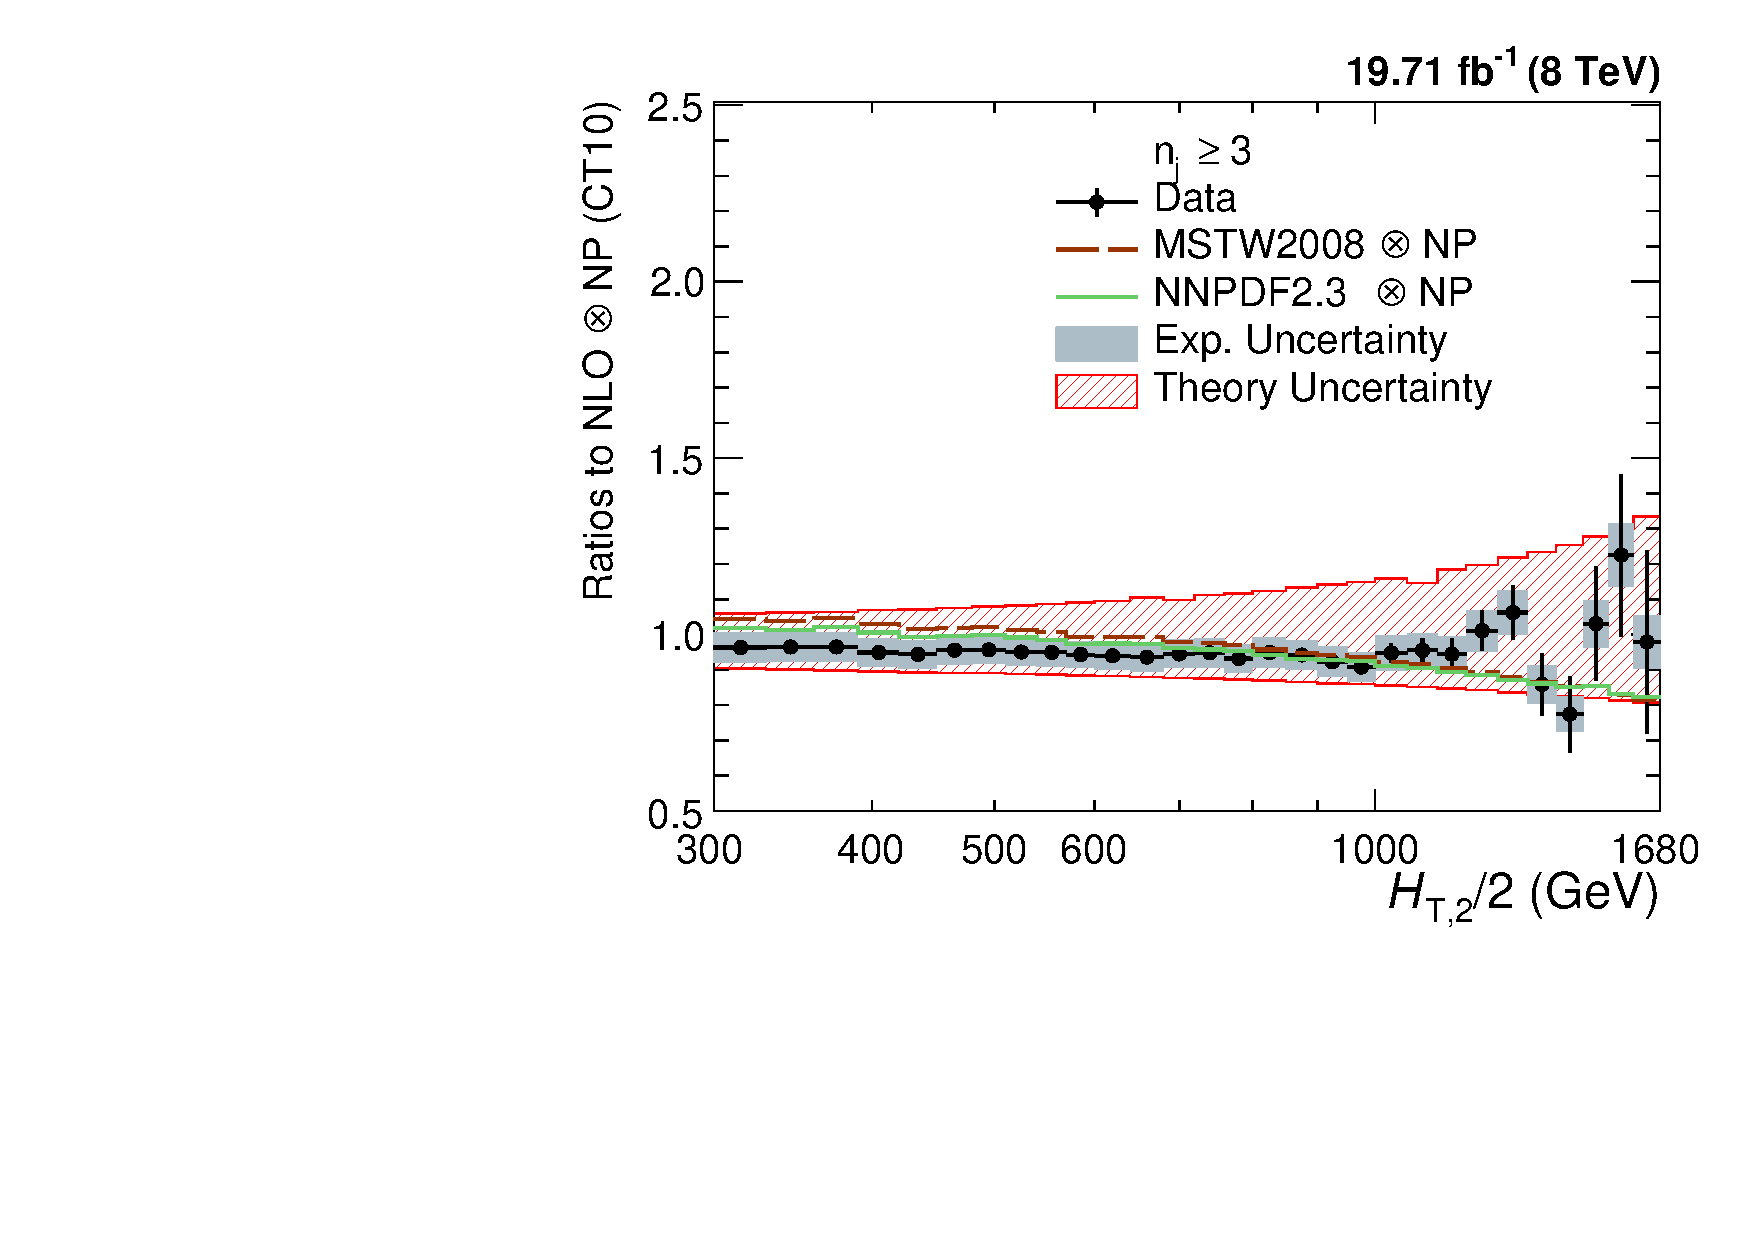
\includegraphics[width=0.5\textwidth]{Plots_HT_2_150/Comparison_data_NLO_Pdfs_3.pdf}\\
  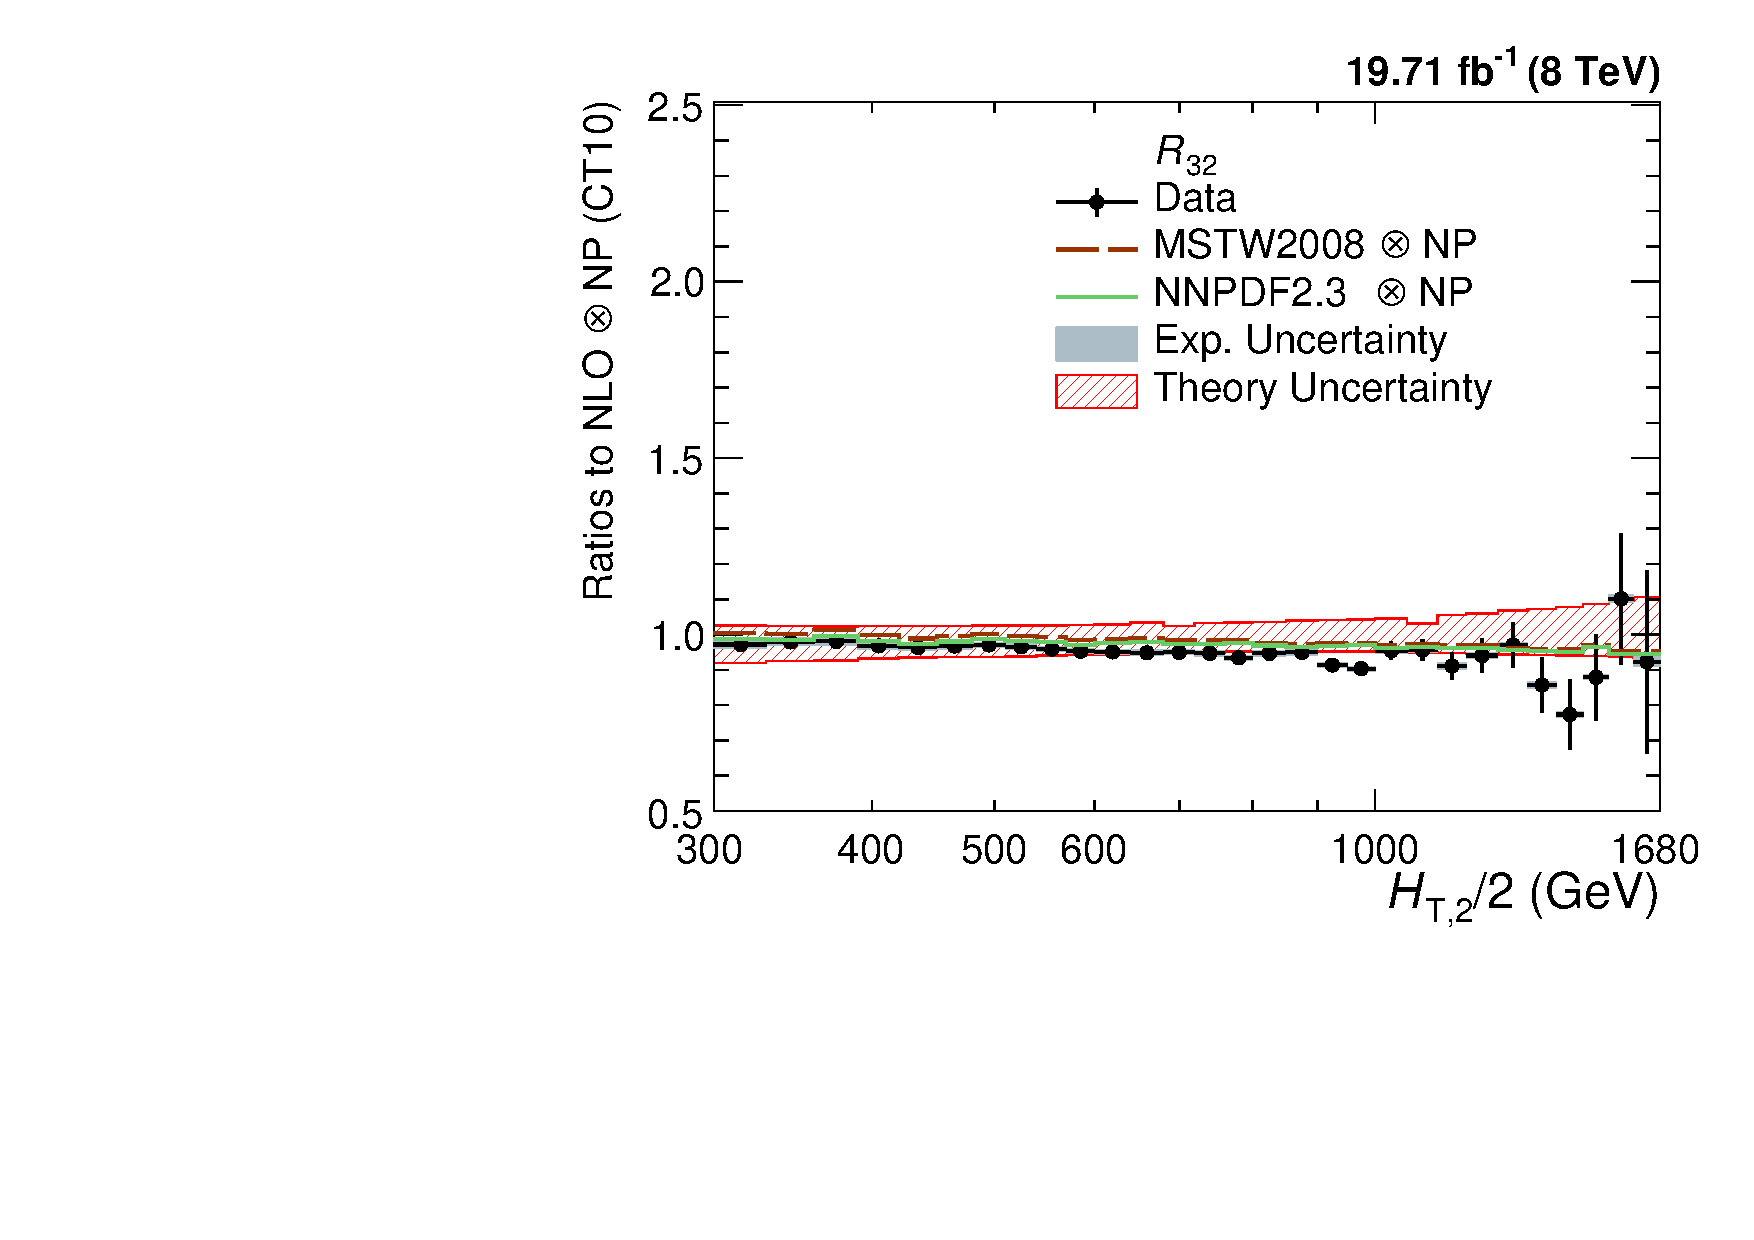
\includegraphics[width=0.5\textwidth]{Plots_HT_2_150/Comparison_data_NLO_Pdfs_ratio_32.pdf}\\  
  \caption{Ratio of data over theory using the CT10 PDF set for
    inclusive 2-jet (top left) and inclusive 3-jet event cross
    sections (top right) and their ratio \ratio (bottom). For comparison predictions employing two
    other PDF sets are also shown. The error bars correspond to the
    statistical uncertainty of the data and the shaded rectangles to
    the total experimental systematic uncertainty. The shaded band
    around unity represents the total uncertainty of the theory.}
  \label{fig:data_NLOPdfs}
\end{center}  
\end{figure}

As for the NP corrections, the \POWHEG framework providing a NLO dijet
calculation matched to the parton showers of \PYTHIAE is used for a
comparison. Here, \POWHEG + \PYTHIAE are employed with the CUETS1 and
CUETM1 tunes. The ratios of data over theory from \POWHEG + \PYTHIAE
with tune CUETS1 are shown in Figure~\ref{fig:data_MC}. For
comparison, the LO prediction from \PYTHIAS, the tree-level multi-leg
improved prediction by \MadGraphF + \PYTHIAS, and the matched NLO
prediction from \POWHEG + \PYTHIAE with tune CUETM1 are shown as
well. Significant discrepancies, which are cancelled to a large extent
in the ratio \ratio, are visible in the comparison with the LO
prediction from \MadGraphF + \PYTHIAS, in particular for small \httwo.
In contrast, the employed dijet MC \PYTHIAE and \POWHEG + \PYTHIAE
better describe the 2-jet event cross section, but fail for the 3-jet
ones. A more satisfactory description can be expected from 3-jet
\POWHEG predictions matched to \PYTHIAE for showering and
hadronization.

\begin{figure}[!htbp]
\begin{center}
  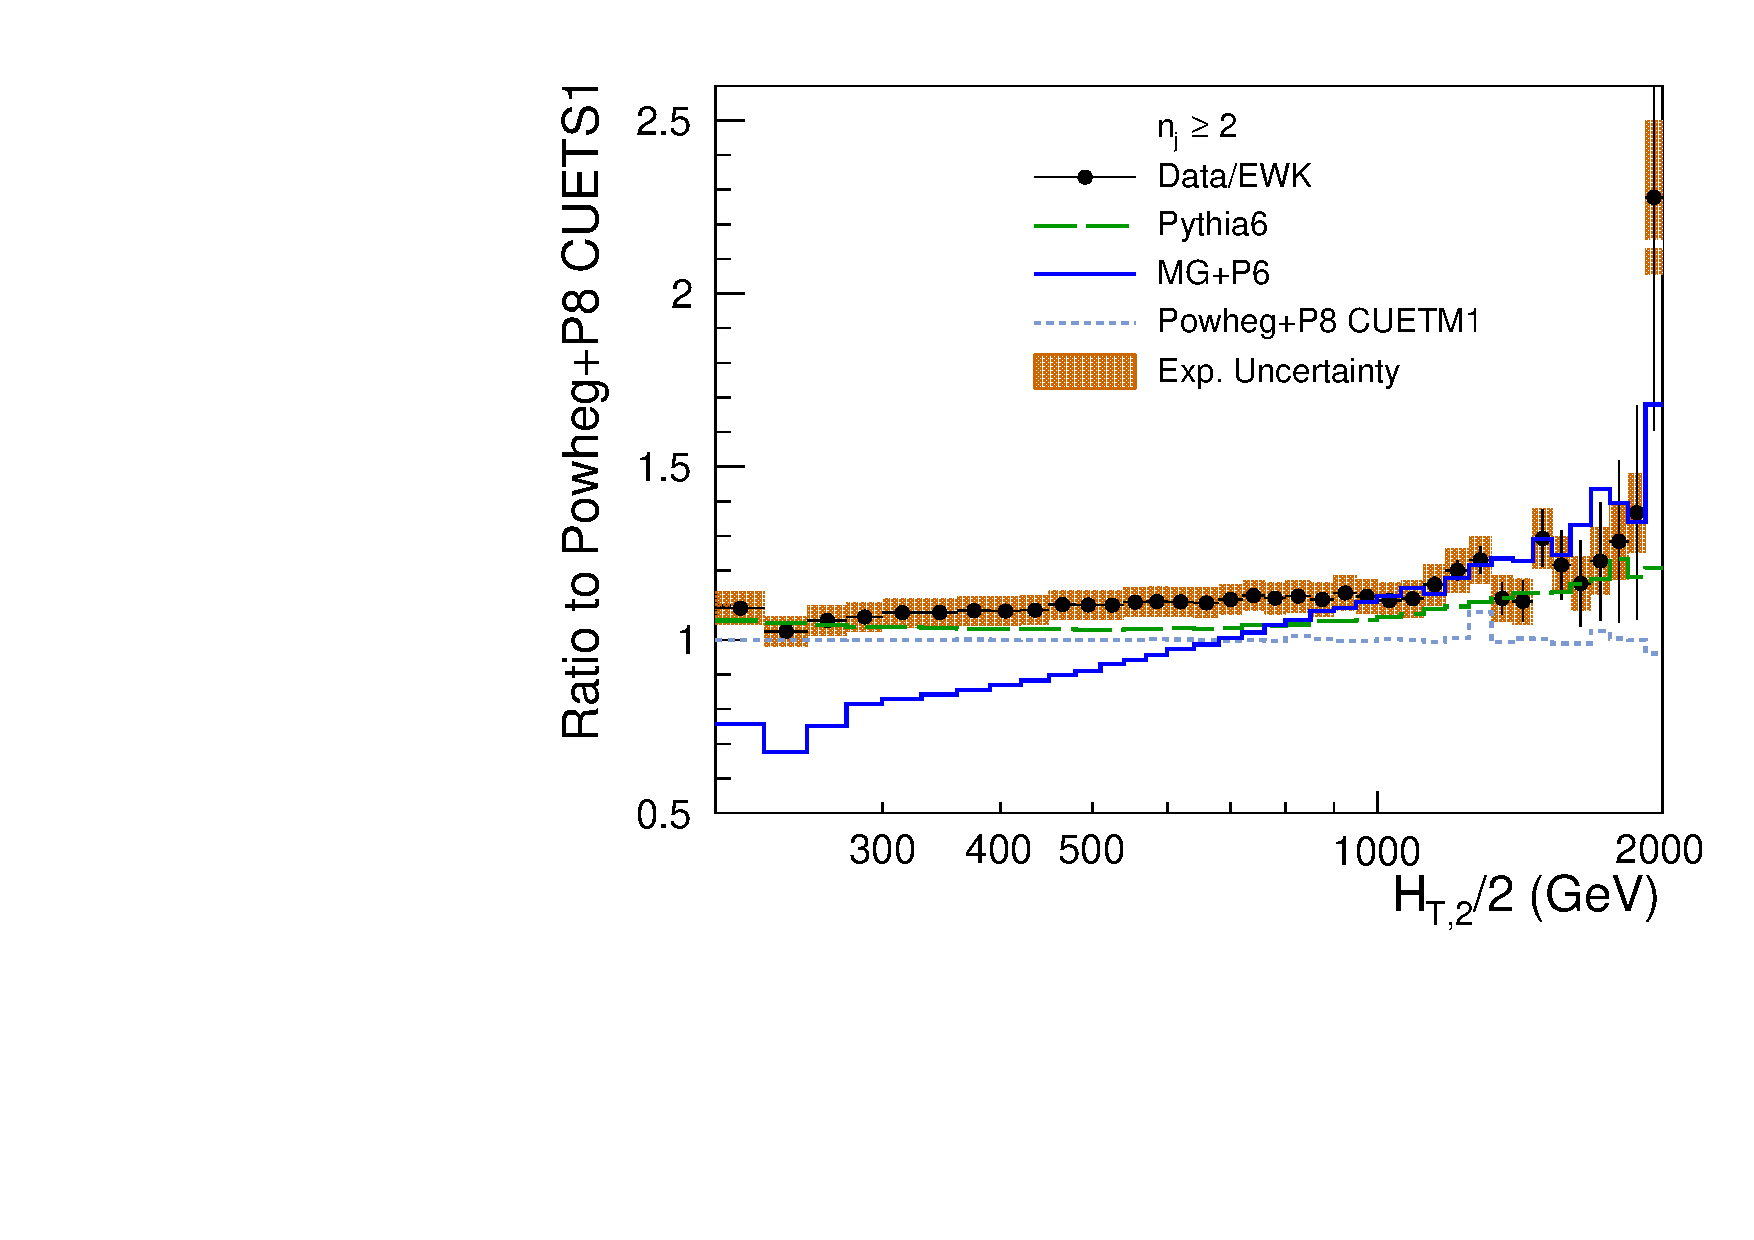
\includegraphics[width=0.5\textwidth]{Plots_HT_2_150/Comparison_data_MC_samples_2_Pow_EWK.pdf}%
  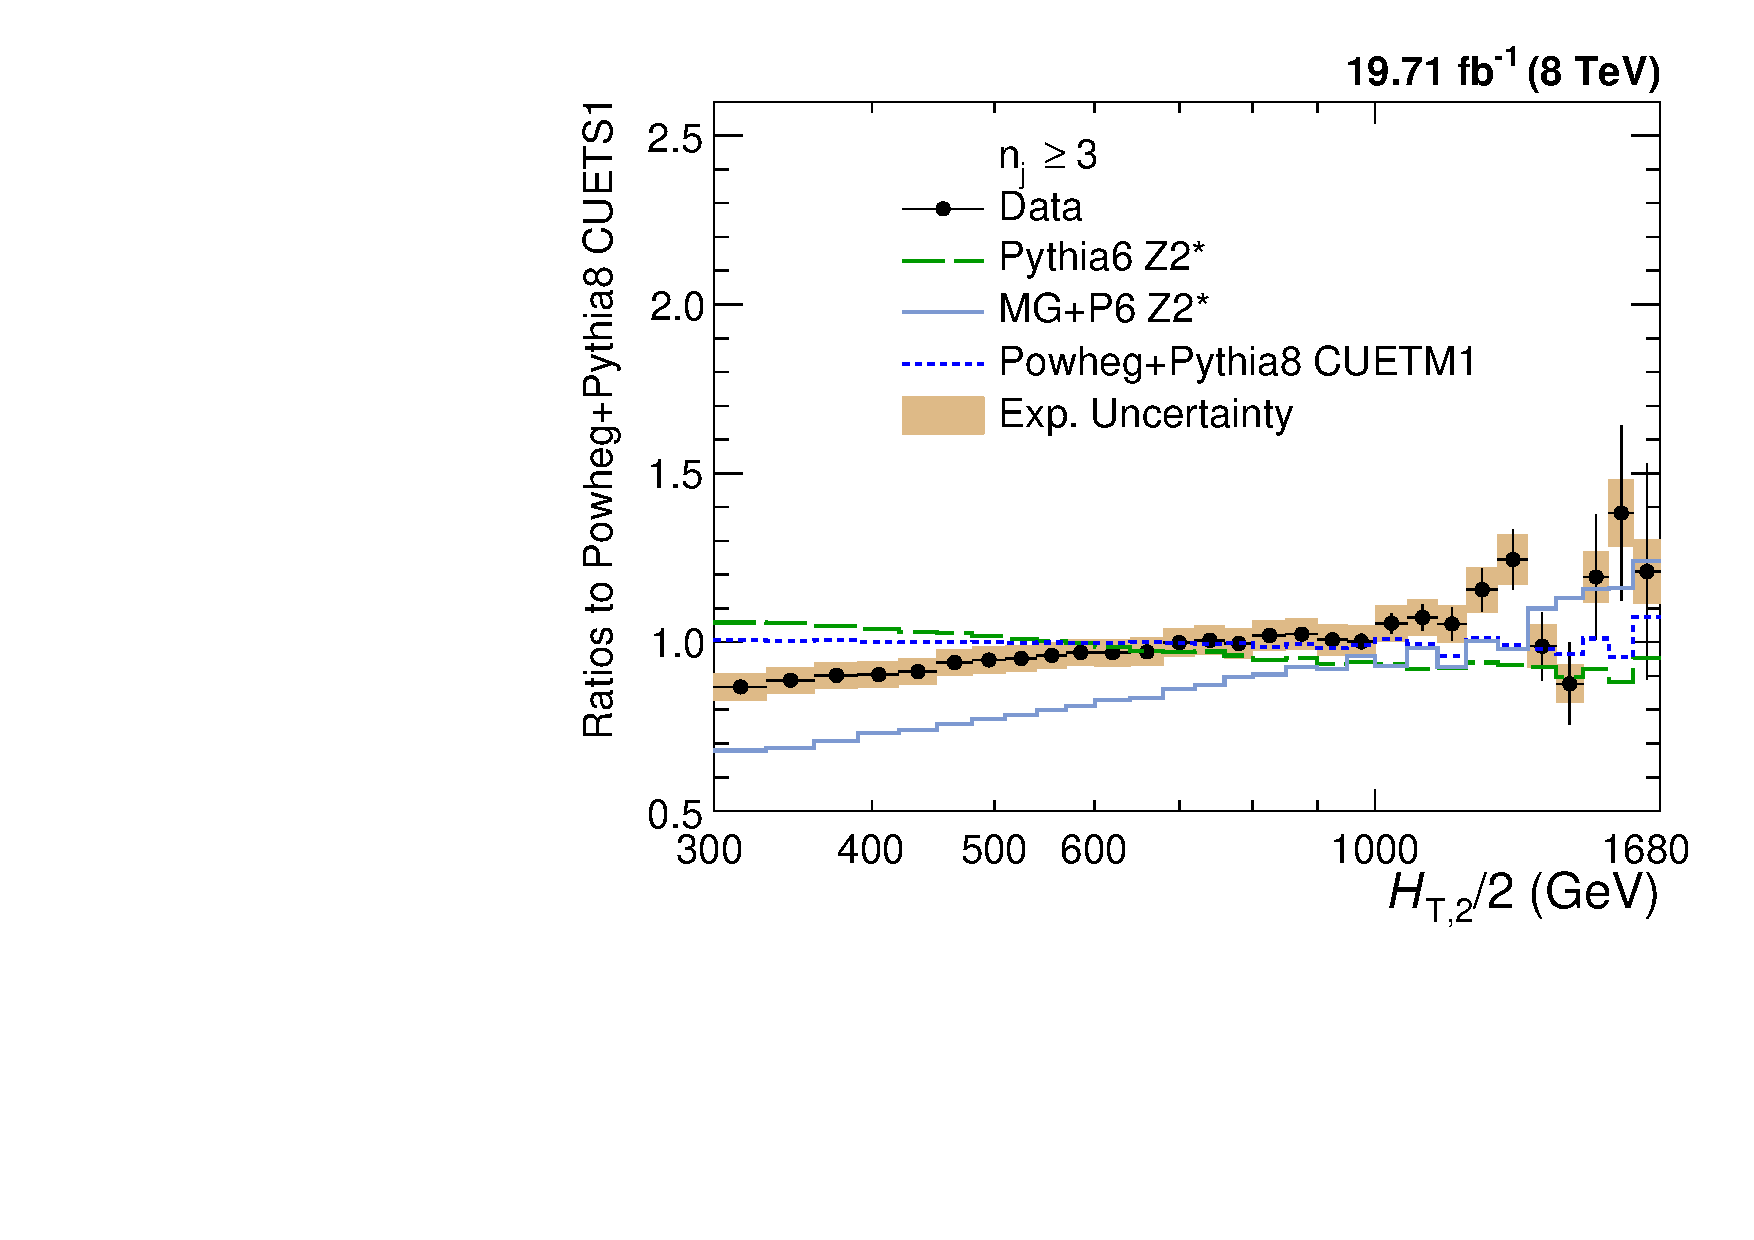
\includegraphics[width=0.5\textwidth]{Plots_HT_2_150/Comparison_data_MC_samples_3_Pow.pdf}\\
  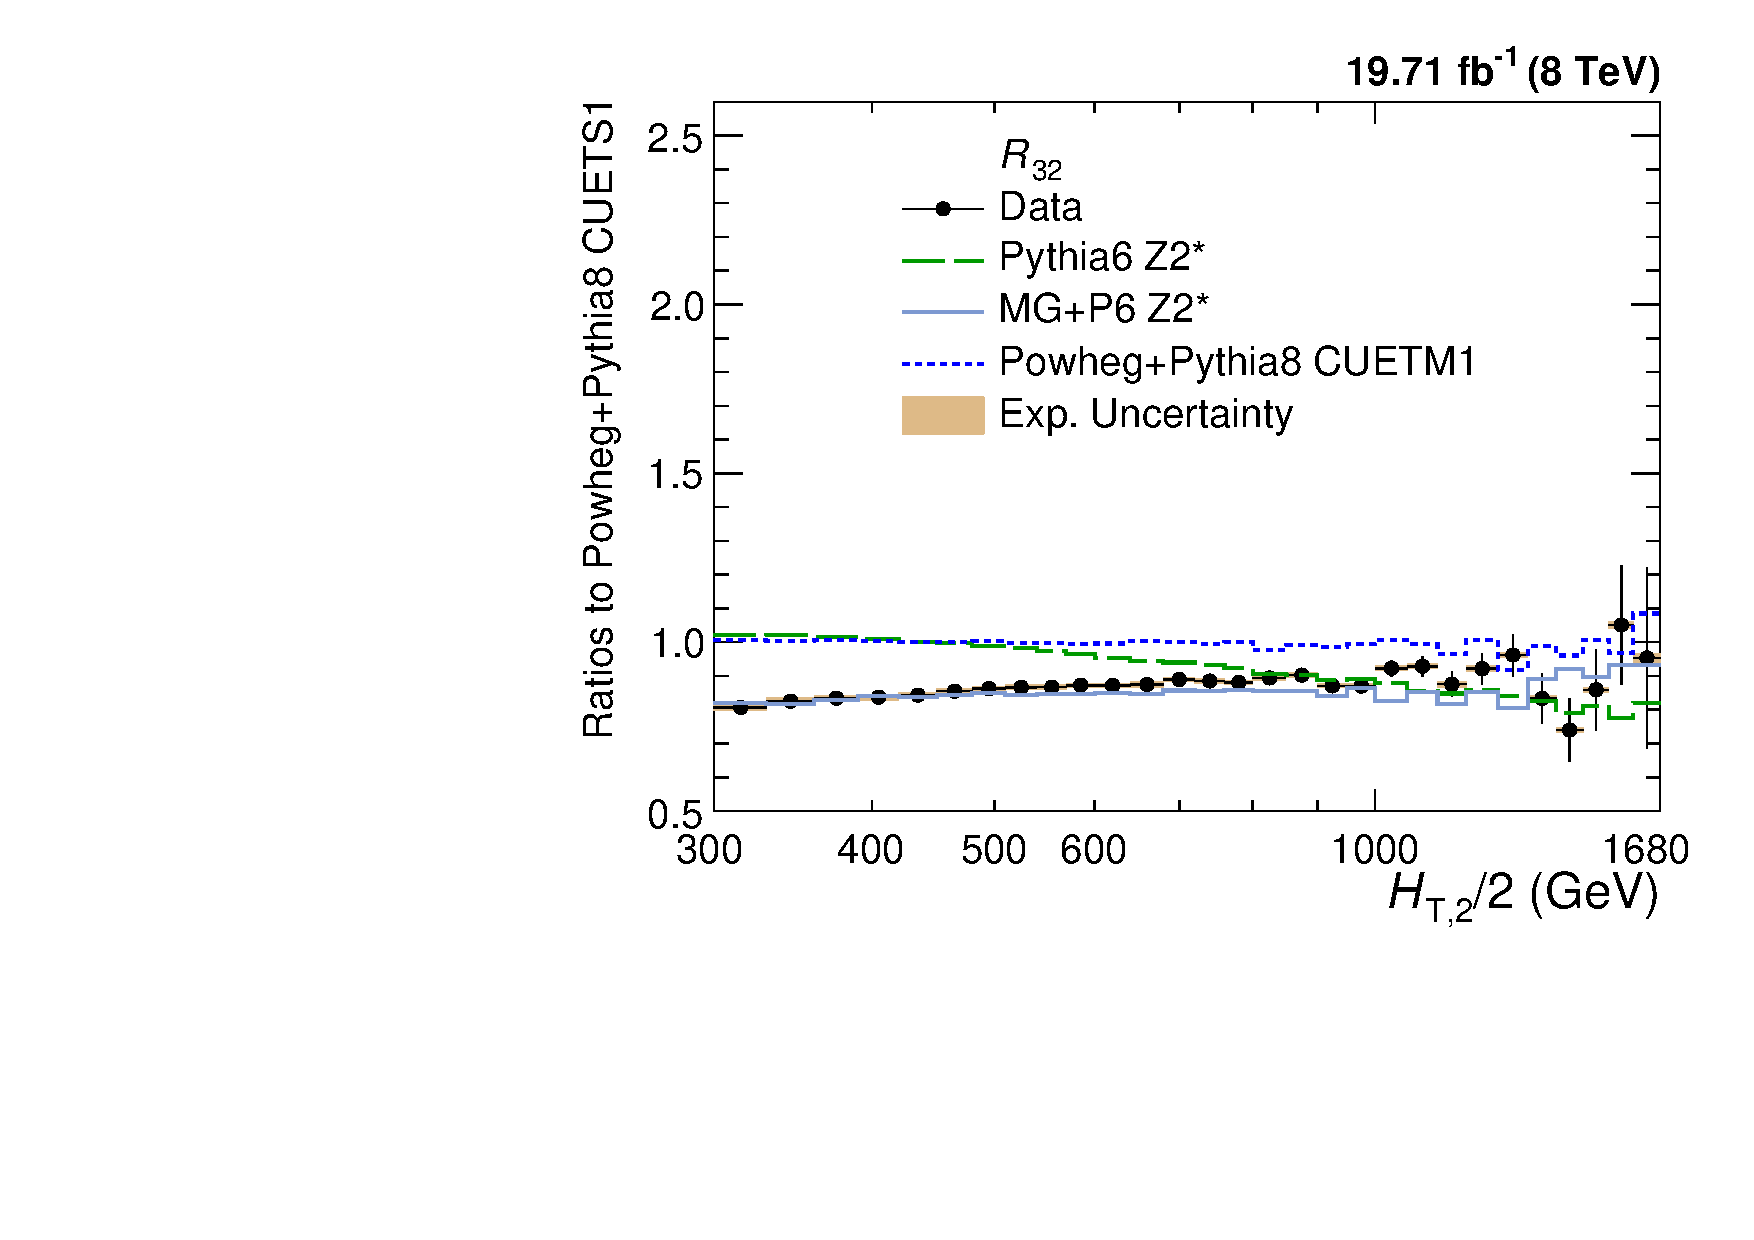
\includegraphics[width=0.5\textwidth]{Plots_HT_2_150/Comparison_data_MC_samples_ratio_32_Pow.pdf}\\
  \caption{Ratio of data over the prediction from \POWHEG + \PYTHIAE
    with tune CUETS1. For comparison the alternative tune CUETM1 of
    \POWHEG + \PYTHIAE, the tree-level multi-leg improved prediction
    by \MadGraphF + \PYTHIAS with tune \Ztwostar, and the the LO MC
    predictions from \PYTHIAS tune \Ztwostar are shown as well. The
    error bars correspond to the statistical uncertainty of the data
    and the shaded rectangles to the total experimental systematic
    uncertainty. EWK corrections have been accounted for in this
    comparison in the 2-jet case.}
  \label{fig:data_MC}
\end{center}  
\end{figure}

Figure~\ref{fig:ratio} presents the cross section ratio \ratio, as obtained from
unfolded cross sections (blue soled circles), in comparison to that from NLO pQCD (CT10 PDF) (red dashed line) and to the ratio
previously measured at 7 \TeV~\cite{Chatrchyan:2013txa}.

\begin{figure}[!htbp]
  \begin{center}
    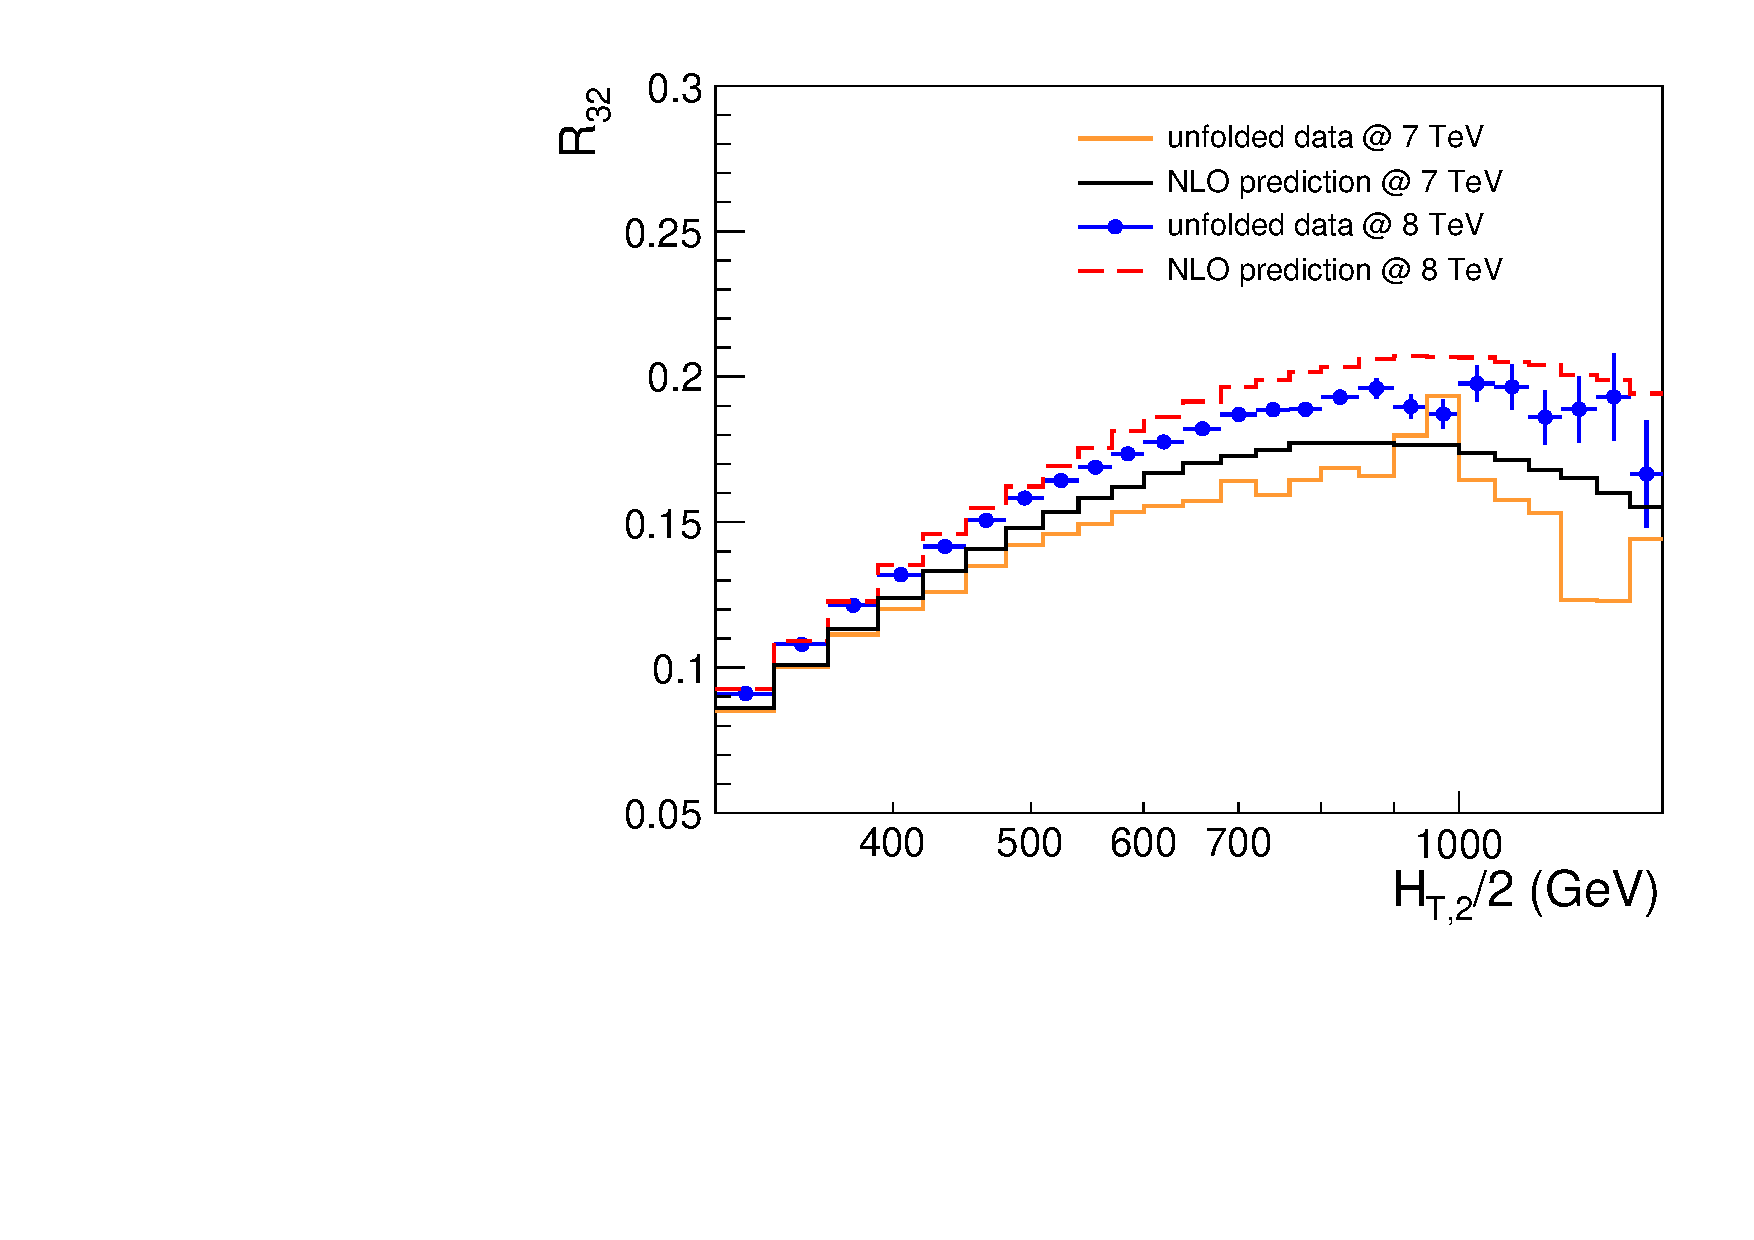
\includegraphics[width=0.50\textwidth]{Plots_HT_2_150/Ratio_32_unfolded_all_7TeV.pdf}
    \caption{Cross section ratios \ratio obtained from unfolded cross sections (blue solid circles), from NLO pQCD (CT10 PDF) (red dashed line), as a function of \httwo in comparison with the previously measured at 7.}
    \label{fig:ratio}
  \end{center}
\end{figure}

\end{comment}
